\documentclass[11pt]{article}

\usepackage[margin=1in]{geometry}
\usepackage{fontspec}
\usepackage{xeCJK}
\setCJKmainfont{Microsoft JhengHei}
\usepackage{amsmath,amssymb}
\usepackage{booktabs}
\usepackage{graphicx}
\usepackage[font=small,labelfont=bf]{caption}
\usepackage{enumitem}
\usepackage[hidelinks]{hyperref}
\usepackage{xurl}
\usepackage{setspace}
\setstretch{1.15}
\setlist{itemsep=2pt,topsep=4pt}
\graphicspath{{../figures/paper/}}

\title{Tracing China in \textit{Lianhe Zaobao}\\[6pt] \large A Computational Study of the China Desk, 2006--2025}
\author{Ethan Yong\\ EAS407, Fall 2025}
\date{}

\begin{document}
\maketitle

\begin{abstract}
\noindent In 2023, \textit{The Washington Post} argued that Singapore's \textit{Lianhe Zaobao} increasingly echoed Beijing's message. This paper asks whether the writing of Zaobao's China desk changed after the December 2021 restructuring of SPH Media, the event most often linked to that claim. I built an index of 618,626 archived Zaobao articles from the Internet Archive and analyze a stratified sample of 28,152 articles from four desks. I compare the China desk with the World, Singapore and Southeast Asia desks in three ways: the rates of hedging, boosting, obligation, permission and attribution words; a classifier that measures how easy it is to tell two desks' writing apart; and an open-vocabulary comparison of the words that set each desk apart. I find no change in tone at the restructuring. The China desk has used roughly a third fewer hedges than the World desk for twenty years, and much of that gap remains when articles on the same topic are compared, so it is not only a result of what the desk covers. At the same time, it hedges more than the Singapore desk and uses fewer obligation words than the World desk. On a style axis fixed before 2021, the China desk has drifted slowly toward the Singapore desk since about 2019, with no break at the restructuring. The clearest change after 2021 is in sourcing. References to official bulletins and official websites on the China desk rose about threefold relative to the World desk, and the increase remains when COVID coverage and the pandemic years are excluded. Over the same period, the share of citations going to Chinese state media fell. I found this pattern while exploring the data, so I present it as a hypothesis for future work rather than a confirmed result.
\end{abstract}

\section{Introduction}

\textit{Lianhe Zaobao} (聯合早報) was founded in March 1983, when Singapore's two main Chinese-language newspapers, \textit{Nanyang Siang Pau} (南洋商報) and \textit{Sin Chew Jit Poh} (星洲日報), merged. It became the city-state's flagship Chinese-language daily, published by the company now called SPH Media \cite{sph100}. Zaobao went online early. Its website launched in August 1995, and SPH describes it as the first Chinese-language newspaper in the world to do so \cite{sphhistory}. The website now runs separate editions for Singaporean, international and mainland Chinese readers \cite{zaobao}, and it is one of the few foreign-owned Chinese-language news sites that readers inside the People's Republic of China can still reach \cite{thinkchina}.

In late 2019, Zaobao launched \textit{ThinkChina}, an English-language site that repackages Zaobao's China coverage for a global audience. In December 2021, SPH moved its media business into SPH Media Trust, a not-for-profit company limited by guarantee \cite{ho2022}. Around the same time, Zaobao's coverage of the Peng Shuai case drew attention. In November 2021, the tennis player Peng Shuai accused the retired Vice Premier Zhang Gaoli of sexual coercion \cite{gan2021}. The accusation was censored in China, and in December Zaobao published an exclusive video interview in which Peng said she had never made a sexual assault allegation \cite{gu2021}. In July 2023, \textit{The Washington Post} published an analysis of more than 700 Zaobao articles and argued that the paper increasingly echoed Beijing's positions on topics such as Hong Kong and Xinjiang \cite{mahtani2023}. Singapore's Ambassador to the United States, Lui Tuck Yew, replied that the article misrepresented Singapore's media and rejected the claim that Zaobao repeats Chinese propaganda \cite{lui2023}.

Most of this debate rests on selected examples. This paper instead measures how the China desk writes across twenty years (2006--2025) and compares it with three other desks of the same newspaper. The comparison desks are needed because Zaobao as a whole changed over this period: its website was redesigned, its house style changed, and so did the news. A change on the China desk is only informative if the other desks did not change in the same way.

\subsection*{Research questions}

The Washington Post's thesis suggests three testable claims about the China desk. I state each as a question and a hypothesis. The hypotheses describe what we would expect to see if the thesis were right.

\begin{enumerate}[label=\textbf{Q\arabic*.}, leftmargin=*]
\item \textbf{Divergence:} Did the China desk's writing pull away from the World desk after the restructuring? \\
\textit{Hypothesis:} China-desk articles become easier to tell apart from World-desk articles after December 2021, because the China desk's writing moves away from that of the World desk.
\item \textbf{Convergence:} Did the China desk move toward the Singapore desk? \\
\textit{Hypothesis:} After December 2021, China-desk articles look more like Singapore-desk articles than they did before.
\item \textbf{Epistemic stance:} Is the China desk more assertive than other desks, and did this change? \\
\textit{Hypothesis:} The China desk uses fewer hedges (``possibly'', ``perhaps'') and more obligation words (``must'', ``should'') than the World desk, and the gap widens after December 2021.
\end{enumerate}

\noindent Where the data show a stable difference between desks, I also ask whether it reflects how the desk writes or simply the topics it covers. Working on these questions led to a fourth, exploratory finding about which sources the China desk cites. I report it separately in Section~\ref{sec:sources}, since I did not plan it in advance.

\section{Data}

\subsection{Building the archive}

All articles come from the Internet Archive's Wayback Machine, which avoids any later edits made on the live website. I queried the Archive's index (the CDX API) for every web address that matches one of Zaobao's three article formats.

\begin{itemize}
\item Legacy desk articles from 2006 to 2012 have addresses such as \nolinkurl{/zg/zg100415_009.shtml}. Here, \texttt{zg} (中國, \textit{zhongguo}) is the China desk, \texttt{gj} (國際, \textit{guoji}, ``international'') the World desk, \texttt{sp} (新加坡, \textit{xinjiapo}) the Singapore desk and \texttt{yx} the Southeast Asia desk.
\item Modern desk articles from 2015 onward have addresses such as \nolinkurl{/news/china/story20200605-1058735}.
\item Realtime (即時, \textit{jishi}) articles come from Zaobao's free instant-news section, with addresses such as \nolinkurl{/realtime/china/story20130523-207775}.
\end{itemize}

Each address contains the publication date, and I date every article by that date. The date on which the Archive first saved a page is a poor substitute: 19\% of modern desk articles in the index were first captured in a later year, sometimes several years after publication. The same article also often appears under several addresses (\texttt{http} and \texttt{https}, \texttt{.com} and \texttt{.com.sg}, or with tracking tags such as \nolinkurl{?utm_source=telegram}), so I reduce each article to one identifier and keep its earliest archived copy. The result is an index of 618,626 unique articles. Of these, 240,745 desk articles and 342,754 realtime articles were published between 2006 and 2025.

\subsection{What the archive contains}

The archive does not hold the same kind of material in every year, and this affects every part of the study (Figure~\ref{fig:data}).

\begin{itemize}
\item \textbf{No desk articles for 2013--2015:} During the site's redesign, the Wayback Machine saved the desks' daily index pages but almost none of their articles. Only 197 desk article addresses exist for these three years, against several thousand per desk in other years. The index pages look like articles at first glance, but each one mixes teasers from every section with the site's footer, so I leave them out.
\item \textbf{Paywall teasers from 2016 to 2023:} Zaobao put much of its desk content behind a subscription. For most of these articles, the archived copy shows only the first paragraph or two, followed by an invitation to subscribe. In my sample, 58.6\% of desk pages from 2016--2025 are teasers, and the rate is between 70\% and 80\% in every year from 2016 to 2022.
\item \textbf{Realtime articles are complete:} The realtime section is free to read, and only 0.2\% of its archived pages are truncated. It covers the China, World and Singapore desks from 2013 to 2025, though not Southeast Asia.
\end{itemize}

\begin{figure}[tbp]
\centering
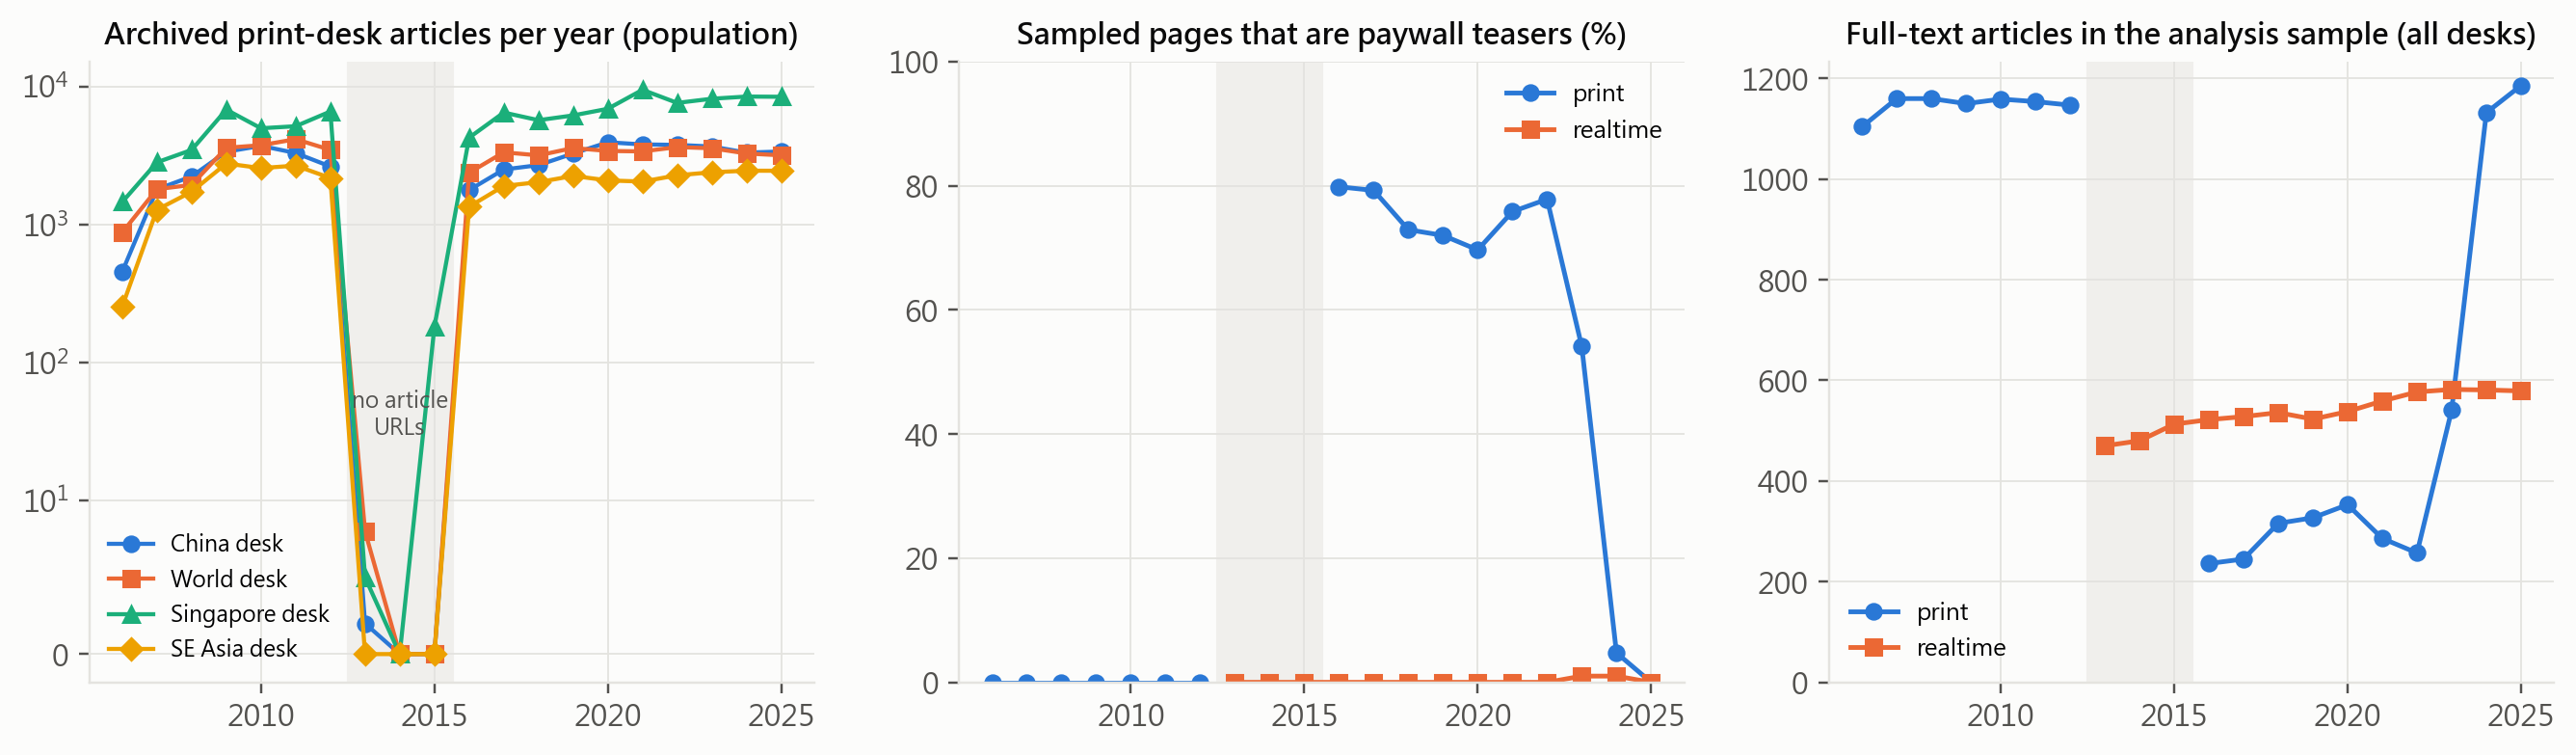
\includegraphics[width=\textwidth]{fig01_archive_coverage.png}
\caption{What the archive holds. The left panel shows archived desk articles per year on a log scale, with almost none for 2013--2015. The middle panel shows the share of sampled pages that are paywall teasers. The right panel shows the number of complete articles in the analysis sample.}
\label{fig:data}
\end{figure}

These gaps mean I cannot follow the full texts of desk articles through the period that matters most. The full texts that do survive for 2016--2023 belong mostly to free articles, which Zaobao chose to leave open, so they are not a random sample. I therefore work with two corpora (Table~\ref{tab:corpora}). The realtime corpus is the main source for 2013--2025, since its texts are complete and unselected. For desk articles, I use the \textit{lead}, meaning the first two paragraphs, which is visible for every article whether or not the article is behind the paywall. I report full-text results for free desk articles only as a secondary check.

\begin{table}[tbp]
\centering
\small
\begin{tabular}{@{}lllll@{}}
\toprule
Corpus & Years & Desks & Text analyzed & Articles \\
\midrule
Desk & 2006--2012 & China, World, Singapore, SE Asia & full text & 8,352 \\
Desk & 2016--2025 & China, World, Singapore, SE Asia & lead (first two paragraphs) & 12,000 \\
Realtime & 2013--2025 & China, World, Singapore & full text & 7,800 \\
\bottomrule
\end{tabular}
\caption{The two corpora. I never compare levels across corpora, since realtime news and desk articles are different genres.}
\label{tab:corpora}
\end{table}

\subsection{Sampling}

I drew a stratified random sample in which each stratum is one corpus, one desk and one publication year. Within each stratum, I put the articles in a random order, with a fixed seed so the draw can be repeated, and downloaded them in that order. After cleaning, I kept the first 300 usable articles in each desk stratum and the first 200 in each realtime stratum. Keeping the first $n$ usable articles of a random order gives a simple random sample of the usable articles, so failed downloads do not bias the sample. The final sample has 28,152 articles, and every stratum is full except the 2006 Southeast Asia desk, which only has 252 usable articles in the archive. Of these articles, 19,901 have complete text.

\subsection{Extracting and cleaning the text}

Each page went through the same steps.

\begin{enumerate}
\item \textbf{Decoding:} I stored the raw bytes of each page and decoded them once, using the character set the page declares. Legacy pages use GB2312, which I read with its superset GB18030.
\item \textbf{Finding the article:} Each version of the site's layout keeps the article body in a known container. I take paragraphs only from that container, which leaves out menus, headlines of other stories and footers.
\item \textbf{Removing boilerplate:} Some text repeats across many pages, such as copyright notices and subscription prompts. I removed any paragraph that appears in five or more different articles, 105 paragraphs in total. This step matters because correspondent bylines such as 于澤遠 北京報道 (``Yu Zeyuan, reporting from Beijing'') repeat on many China-desk articles, and the word 報道 (\textit{baodao}, ``report'') in them would otherwise count as an attribution marker.
\item \textbf{Flagging teasers:} I flag a page as truncated when its article container holds a subscription prompt. In the 2016--2019 layout, a real paywall prompt (登錄 $|$ 免費試閱14天 $|$ 開始訂閱, ``log in, free trial, subscribe'') looks similar to a promotional line added to the end of complete articles (想閱讀更多新聞？, ``want to read more news?''), and I treat only the first as a sign of truncation.
\item \textbf{Exclusions:} I dropped pages that failed to download (63), legacy print-edition teasers that only say the full story is in that day's paper (319), pages with fewer than 50 Chinese characters of text (1,755) and exact duplicates (6).
\end{enumerate}

\noindent To check the extraction, I read 40 randomly chosen extracted articles drawn from every era. All of them were article prose. In a few layouts, the first extracted paragraph is the headline or a subheading, so a lead sometimes includes one; this affects all desks alike.

\section{Methods}

\subsection{Words and markers}

I converted all text to simplified Chinese with OpenCC and split it into words with the jieba segmenter \cite{jieba}, which works more reliably on simplified text. I give Chinese examples in this paper in traditional characters. I count only words that contain at least one Chinese character, so punctuation, numbers and English names do not change the rates. For each article, $n_i$ is its number of words.

The first measure is a set of marker words for epistemic and deontic modality, based on Palmer's classification \cite{palmer} and on Hyland's work on hedges and boosters \cite{hyland}. The markers fall into five categories (Table~\ref{tab:lexicon}). A word only counts when the segmenter produces it as a whole word. This matters in Chinese, where many markers are also parts of longer words. 據 (\textit{ju}, ``according to'') appears inside 數據 (\textit{shuju}, ``data''), and 說 (\textit{shuo}, ``say'') appears inside 說明 (\textit{shuoming}, ``explain''), so counting substrings would mix unrelated words into the attribution category. Fixed phrases such as 據報道 (\textit{ju baodao}, ``it is reported'') are kept as one word, so they count once. I include boosters as well as hedges, since a fall in hedging can mean either less caution or more assertion, and only measuring both can tell the two apart.

\begin{table}[tbp]
\centering
\small
\begin{tabular}{@{}llp{0.6\textwidth}@{}}
\toprule
Category & What it marks & Examples \\
\midrule
Hedge & possibility, uncertainty & 可能 (\textit{keneng}, possibly), 可能性 (\textit{kenengxing}, possibility), 或許 (\textit{huoxu}, perhaps), 也許 (\textit{yexu}, maybe), 似乎 (\textit{sihu}, seemingly), 估計 (\textit{guji}, estimate), 不排除 (\textit{bu paichu}, cannot rule out) \\
\addlinespace
Booster & certainty & 顯然 (\textit{xianran}, obviously), 無疑 (\textit{wuyi}, undoubtedly), 確實 (\textit{queshi}, indeed), 必然 (\textit{biran}, inevitably), 勢必 (\textit{shibi}, bound to), 毫無疑問 (\textit{haowu yiwen}, without doubt) \\
\addlinespace
Obligation & necessity, duty & 必須 (\textit{bixu}, must), 應當 (\textit{yingdang}, ought to), 應該 (\textit{yinggai}, should), 不得 (\textit{bude}, must not), 有必要 (\textit{you biyao}, it is necessary) \\
\addlinespace
Permission & permission & 可以 (\textit{keyi}, may), 允許 (\textit{yunxu}, allow), 准許 (\textit{zhunxu}, permit), 獲准 (\textit{huozhun}, be permitted), 有權 (\textit{youquan}, have the right) \\
\addlinespace
Attribution & reporting a source & 據 (\textit{ju}, according to), 據悉 (\textit{juxi}, it is learned), 據報道 (\textit{ju baodao}, it is reported), 表示 (\textit{biaoshi}, said), 指出 (\textit{zhichu}, pointed out), 稱 (\textit{cheng}, claimed), 說 (\textit{shuo}, say), 認為 (\textit{renwei}, believe), 強調 (\textit{qiangdiao}, stress), 透露 (\textit{toulu}, reveal) \\
\bottomrule
\end{tabular}
\caption{Marker categories, with the most frequent words in each. Two words are ambiguous. 應該 (\textit{yinggai}) can mean ``should'' or ``probably'', and 可以 (\textit{keyi}) can mean ``may'' or ``can''. Because each word is also analyzed separately (Figure~\ref{fig:terms}), readers can discount these two.}
\label{tab:lexicon}
\end{table}

\subsection{Comparing marker rates between desks}

For one category and two desks, the quantity of interest is the rate ratio
\[
\text{IRR} = \frac{\text{markers per word on the China desk}}{\text{markers per word on the comparison desk}}.
\]
An IRR of 1 means no difference, 0.5 means the China desk uses the markers half as often, and 2 means twice as often. I estimate it with a Poisson regression of each article's marker count $y_i$ on a China-desk indicator and year fixed effects $\gamma$, with $\log n_i$ as an offset,
\[
\log \mathbb{E}[y_i] = \log n_i + \beta_0 + \beta_1\,\text{China}_i + \gamma_{\text{year}(i)}, \qquad \text{IRR} = e^{\beta_1},
\]
so the two desks are always compared within the same years. Word counts in news are overdispersed. Many articles have no hedges at all, and a few have many. The Poisson estimate of $\beta_1$ stays consistent under overdispersion as long as the mean is modeled correctly, and robust (HC1) standard errors keep the confidence intervals valid \cite{wooldridge,santos}. I also fit negative binomial models as a check. When I compare desks within a single year, I only report a ratio if each desk has at least five markers of that category that year, since a ratio built on one or two words is not meaningful.

\subsection{Testing for a break at the restructuring}

To test whether the China desk changed after December 2021, I use a difference-in-differences model that compares the China desk with the World desk before and after the change,
\[
\log \mathbb{E}[y_i] = \log n_i + \alpha_{\text{desk}(i)} + \gamma_{\text{year}(i)} + \delta\,(\text{China}_i \times \text{After}_i),
\]
where $\text{After}_i = 1$ for articles published on or after 1 December 2021. The year effects $\gamma$ absorb everything that changed across the whole newspaper, such as a new house style. The quantity $e^{\delta}$ is how much the China/World ratio changed after the restructuring, and a value of 1 means no change.

I assess $\delta$ in two ways. The first treats articles as independent. The second allows for news events that affect one desk in one year, such as the start of the war in Ukraine for the World desk in 2022. Articles from that year share the same shock, and with only about ten years of data a few such shocks can produce a false break. For this second test, I compute one China/World rate ratio per year and compare the years after 2021 with the earlier years using a Welch $t$-test on the yearly log ratios. I call a change robust only if it holds at both levels.

Finally, I move the break to 1 December of each year from 2014 to 2024 (2017 to 2024 for desk leads, which start in 2016). These placebo breaks show whether December 2021 stands out. If the estimate is just as large when the break is placed in another year, the data show a gradual trend or noise, not a change linked to the restructuring.

\subsection{Is a difference about voice or about topic?}

The World desk covers wars, elections and markets, stories that may invite speculation, while the China desk covers policy announcements and domestic news. A difference in marker rates could therefore reflect subject matter rather than voice. To separate the two, I fit a topic model, non-negative matrix factorization \cite{nmf} of the articles' TF-IDF vectors, on all desks together and without desk labels, and assign each article its dominant topic. I then add topic fixed effects to the rate-ratio model, so that China-desk articles are compared only with World-desk articles on the same topic. I report 20 and 40 topics, and a version restricted to topics in which each desk supplies at least 20\% of the articles, so that only topics both desks actually cover are compared.

\subsection{Measuring how far apart two desks are}

I measure the distance between desks in two ways. The first compares vocabulary as a whole. I represent each article by TF-IDF weights for the 5,000 most common words, which weight a word by how often it appears in the article and by how rare it is across the corpus. For each year, I split each desk's articles at random into two halves and compute the cosine similarity between the average vectors of half of the China desk and half of the World desk. Two samples from the same desk never match perfectly, so I also compare two halves of the China desk with each other as a reference. The distance between the desks is the gap between these two numbers, and repeating the split 200 times gives its range. A cosine between the desks' average rates of the marker categories would not work here. Attribution words are about ten times as frequent as the other markers (20.6 per 1,000 words, against 0.9--1.9), so they make up 99\% of the vector's squared length, and the cosine is about 0.999 even between two random halves of the same desk.

Content similarity mixes what the desks cover with how they write. The second measure focuses on style. For each year and each pair of desks, I train a logistic regression to predict which of the two desks wrote an article and measure its accuracy with the area under the ROC curve (AUC) on articles the model has not seen, using five-fold cross-validation repeated three times. An AUC of 0.5 means the desks are indistinguishable, and 1.0 means they are perfectly separable. I use two sets of features.

\begin{itemize}
\item \textbf{Style:} The relative frequencies of the 300 most common function words, meaning adverbs, conjunctions, prepositions and particles such as 的 (\textit{de}, possessive particle), 也 (\textit{ye}, ``also''), 將 (\textit{jiang}, ``will''), 並 (\textit{bing}, ``and''), 但 (\textit{dan}, ``but''), 據 (\textit{ju}, ``according to'') and 則 (\textit{ze}, ``then''). These words reflect how a text is written much more than what it is about. I left out pronouns and words of place, since they reveal the topic. 我國 (\textit{woguo}, ``our country'') and 本地 (\textit{bendi}, ``local'', meaning Singapore) would let the model use subject matter.
\item \textbf{Full vocabulary:} The TF-IDF weights described above, which mix topic and style.
\end{itemize}

\noindent Four choices keep the AUCs comparable across years. I chose the model's regularization once and then held it fixed. I fitted the scaling of features inside each training fold, so the test articles are never used to fit any part of the model. I used at most 150 randomly chosen articles per desk in every cell, since a classifier trained on more data scores higher for that reason alone. And because a single random draw of 150 articles makes the AUC depend on which articles were drawn (its standard deviation across draws is up to 0.03), every cell averages ten independent draws. Confidence intervals come from bootstrap resamples of the test predictions; they ignore the variability of refitting the model, so they are slightly too narrow.

\subsection{Which desk moved?}

AUC is symmetric: if China and World articles become easier to tell apart, AUC cannot say which desk changed. To find out, I train the China-versus-World classifier, and separately the China-versus-Singapore classifier, only on articles published before December 2021. The classifier's score then places every article, before and after 2021, on a fixed style axis between the two desks. I split the pre-2021 articles into five folds. Each pre-2021 article is scored by the model trained on the other four folds, and each later article by the average of the five fold models. Scoring the later articles with one model retrained on all the earlier ones would be a mistake: a regularized model trained on more data has larger coefficients (here by about 12\%), which would push later China articles toward one end of the axis and later World articles toward the other, and would show a divergence that does not exist. I scale the scores so that the pre-2021 average of the China desk is 1 and that of the other desk is 0.

A desk can also drift slowly for years, and a simple before-and-after comparison would mistake that drift for a break. I therefore fit an interrupted time series for each desk's article scores $s_i$,
\[
s_i = b_0 + b_1\,(t_i - t^{*}) + b_2\,\text{After}_i + \varepsilon_i,
\]
where $t_i$ is the publication date in years and $t^{*}$ is 1 December 2021. The slope $b_1$ is the drift that already existed, and $b_2$ is the jump at December 2021 beyond that drift. Articles from the same year share news shocks, so standard errors are clustered by year, with $t$ critical values on 12 degrees of freedom \cite{cameron}.

A change in house style moves both desks the same way along the axis. What Q1 and Q2 ask about is therefore the \textit{distance} between the desks on the axis. For each year, I compute $D_y$, the China desk's average score minus the other desk's, which averages 1 before 2021. I fit the same trend-and-jump model to the 13 yearly values. Divergence from the World desk (Q1) predicts a positive jump on the China--World axis, and convergence on the Singapore desk (Q2) a negative jump on the China--Singapore axis.

\subsection{Distinctive words}

To see what changed in content without choosing words in advance, I compare word frequencies with the weighted log-odds ratio and an informative Dirichlet prior \cite{monroe}. For word $w$ in groups $i$ and $j$,
\[
\hat\delta_w = \log\frac{y_{wi} + a_w}{n_i + a_0 - y_{wi} - a_w} - \log\frac{y_{wj} + a_w}{n_j + a_0 - y_{wj} - a_w},
\qquad z_w = \frac{\hat\delta_w}{\sqrt{1/(y_{wi}+a_w) + 1/(y_{wj}+a_w)}},
\]
where $y_{wi}$ is the count of $w$ in group $i$, $n_i$ is the group's total word count, and $a_w$ is a prior proportional to the word's frequency in the whole corpus ($a_0 = 10{,}000$). The prior pulls rare words toward zero, so the lists are not dominated by names that appear once or twice. I compare the China and World desks before and after December 2021, and each desk with its own past. With thousands of words, I read the rankings descriptively rather than as individual tests.

\subsection{Sources (exploratory)}

The distinctive words pointed to a change in sourcing, so I counted the names of outlets and official channels. I sorted them into six groups.

\begin{itemize}
\item Chinese state media, such as 新華社 (Xinhua News Agency), 中新社 (China News Service), 人民日報 (\textit{People's Daily}), 央視 (CCTV) and 環球時報 (\textit{Global Times})
\item other mainland media, such as 財新 (Caixin) and 澎湃 (\textit{The Paper})
\item official channels, namely 官網 (\textit{guanwang}, ``official website'') and 通報 (\textit{tongbao}, ``official bulletin'')
\item Taiwanese media
\item Hong Kong media
\item international wires and media
\end{itemize}

\noindent I report how often each group appears per 10,000 characters and its share of all named media citations. For official channels, I also fit the difference-in-differences model with placebo breaks described above, and I check it against the most obvious alternative explanations: I drop articles that mention COVID, drop the pandemic years 2020--2022 entirely, and repeat the test at the level of years. I chose this analysis after seeing the data, so it can suggest hypotheses but cannot confirm them.

\subsection{Multiple comparisons}

This study runs many tests, and some will pass the 0.05 threshold by chance. I group the tests into families defined before looking at the results and control the false discovery rate within each family with the Benjamini--Hochberg procedure \cite{bh}. I report the resulting $q$-values next to the $p$-values. The families are the realtime difference-in-differences tests (five categories), the lead-based ones (five), the AUC change tests (eight), the tests of which desk moved (six) and the source tests (eleven, exploratory). Article-level and year-level tests are corrected separately.

\section{Results}

\subsection{Divergence and convergence (Q1 and Q2)}

The two desks' vocabularies did grow apart, but earlier than the restructuring (Figure~\ref{fig:content}). In the realtime corpus, the similarity between half of the China desk and half of the World desk is 0.64--0.74, against 0.82--0.87 between two halves of the China desk. The gap between the two lines grows from about 0.10 in 2013--2015 to 0.16--0.21 from 2018 onward, three years before the restructuring. This measure reflects what the desks cover as much as how they write, so it cannot say on its own whether the China desk's voice changed.

\begin{figure}[tbp]
\centering
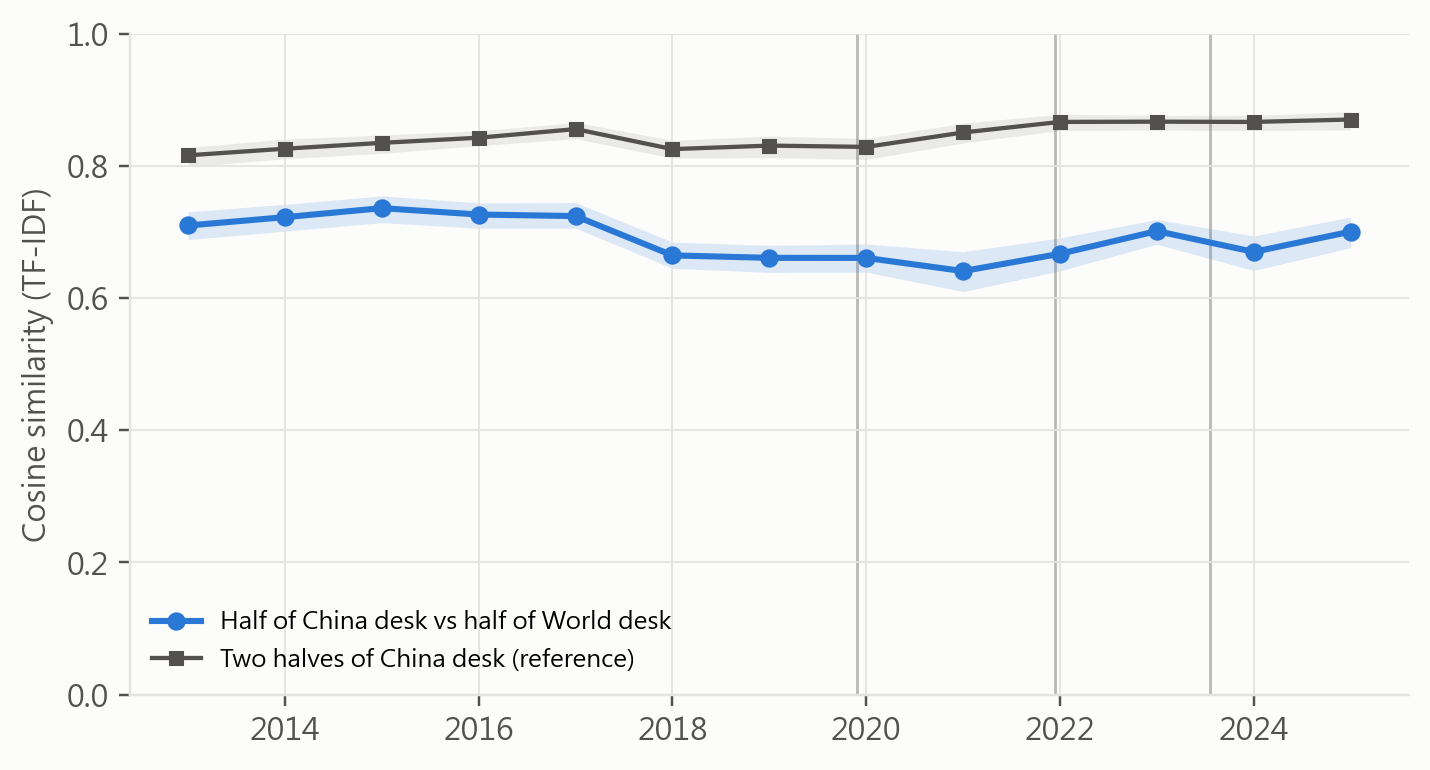
\includegraphics[width=0.75\textwidth]{fig02_content_similarity.png}
\caption{Content similarity between the China and World desks, realtime corpus. The blue line is the cosine similarity between the average TF-IDF vectors of half of the China desk and half of the World desk. The grey line compares two halves of the China desk and serves as a reference. Bands show the middle 95\% of 200 random splits.}
\label{fig:content}
\end{figure}

Function words largely separate style from subject matter, and by this measure the China desk's style is distinctive in every year (Figure~\ref{fig:auc}). Using function words alone, a classifier tells realtime China-desk articles from World-desk articles with an AUC of 0.72--0.80 in every year from 2013 to 2021, and from Singapore-desk articles with an AUC of 0.85--0.92. In the legacy desk corpus, the AUCs are similar (0.81--0.87 against the World desk). With the full vocabulary, the desks are almost perfectly separable (AUC above 0.92), as expected, since the China desk writes about China.

\begin{figure}[tbp]
\centering
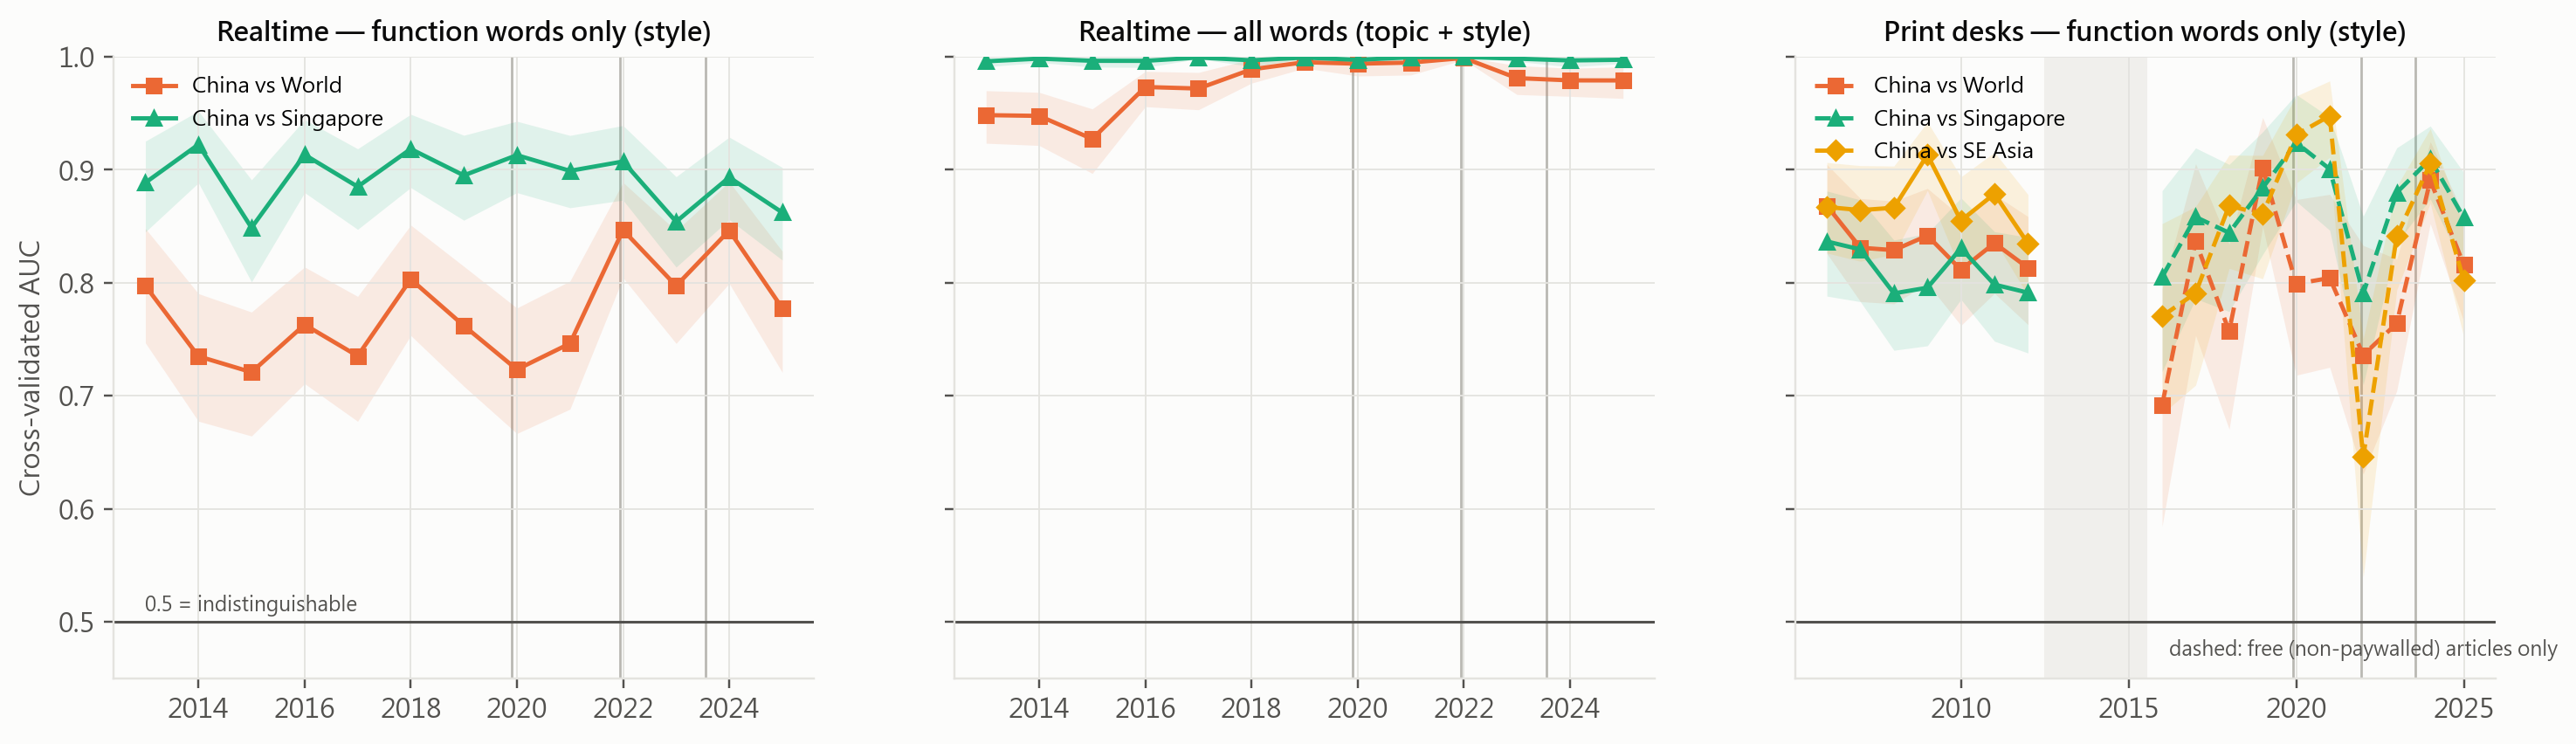
\includegraphics[width=\textwidth]{fig03_desk_distinguishability_auc.png}
\caption{Cross-validated AUC for telling China-desk articles from those of other desks, where 0.5 means indistinguishable. Each point averages ten random draws of up to 150 articles per desk. The left panel uses realtime articles and function words only, the middle panel realtime articles and the full vocabulary, and the right panel desk articles and function words only. The dashed lines after 2016 use free articles only and are less reliable. Vertical lines mark the launch of \textit{ThinkChina}, the SPH restructuring and the \textit{Washington Post} report. Bands are 95\% bootstrap intervals.}
\label{fig:auc}
\end{figure}

After 2021, the realtime China and World desks became somewhat easier to tell apart. The average AUC rose from 0.75 in 2013--2021 to 0.82 in 2022--2025 ($p = 0.026$), but this does not survive the correction for multiple tests ($q = 0.21$). The China--Singapore AUC did not change significantly (0.90 before, 0.88 after, $q = 0.92$). None of the changes in the desk corpus is significant.

On the fixed China--World axis (Figure~\ref{fig:moved} and Table~\ref{tab:moved}), \textit{both} desks moved in the same direction after 2021: the China desk by $-0.14$ of the pre-2021 gap and the World desk by $-0.18$. A shared shift like this is what a paper-wide change in house style would produce, and the distance between the desks did not change (1.00 before, 1.05 after; jump $+0.13$, 95\% CI $-0.14$ to $0.40$). The rise in AUC therefore does not come from the China desk becoming more different in the ways that separated the desks before 2021. If the rise is real, the desks differ after 2021 in new ways, which a classifier refitted each year can detect. This would be expected when the World desk's news changed, with the wars in Ukraine and Gaza.

The China--Singapore axis shows a different pattern. Here, the China desk moved toward the Singapore end ($-0.14$ of the gap) while the Singapore desk stayed where it was ($+0.01$), so the distance between them shrank by about 15\%, from 1.00 to 0.85. But the shrinking began before the restructuring: the distance fluctuated around 1 until 2019, fell to 0.95 in 2020 and 0.88 in 2021, and stayed between 0.81 and 0.89 afterwards. There is no jump at December 2021 ($-0.06$, 95\% CI $-0.20$ to $0.08$), and none of the six tests in this family is significant ($q \ge 0.43$). The China desk's position fell on both axes, so the change is best read as its style becoming gradually less distinctive, not as a turn toward Singapore at a particular moment.

\begin{figure}[tbp]
\centering
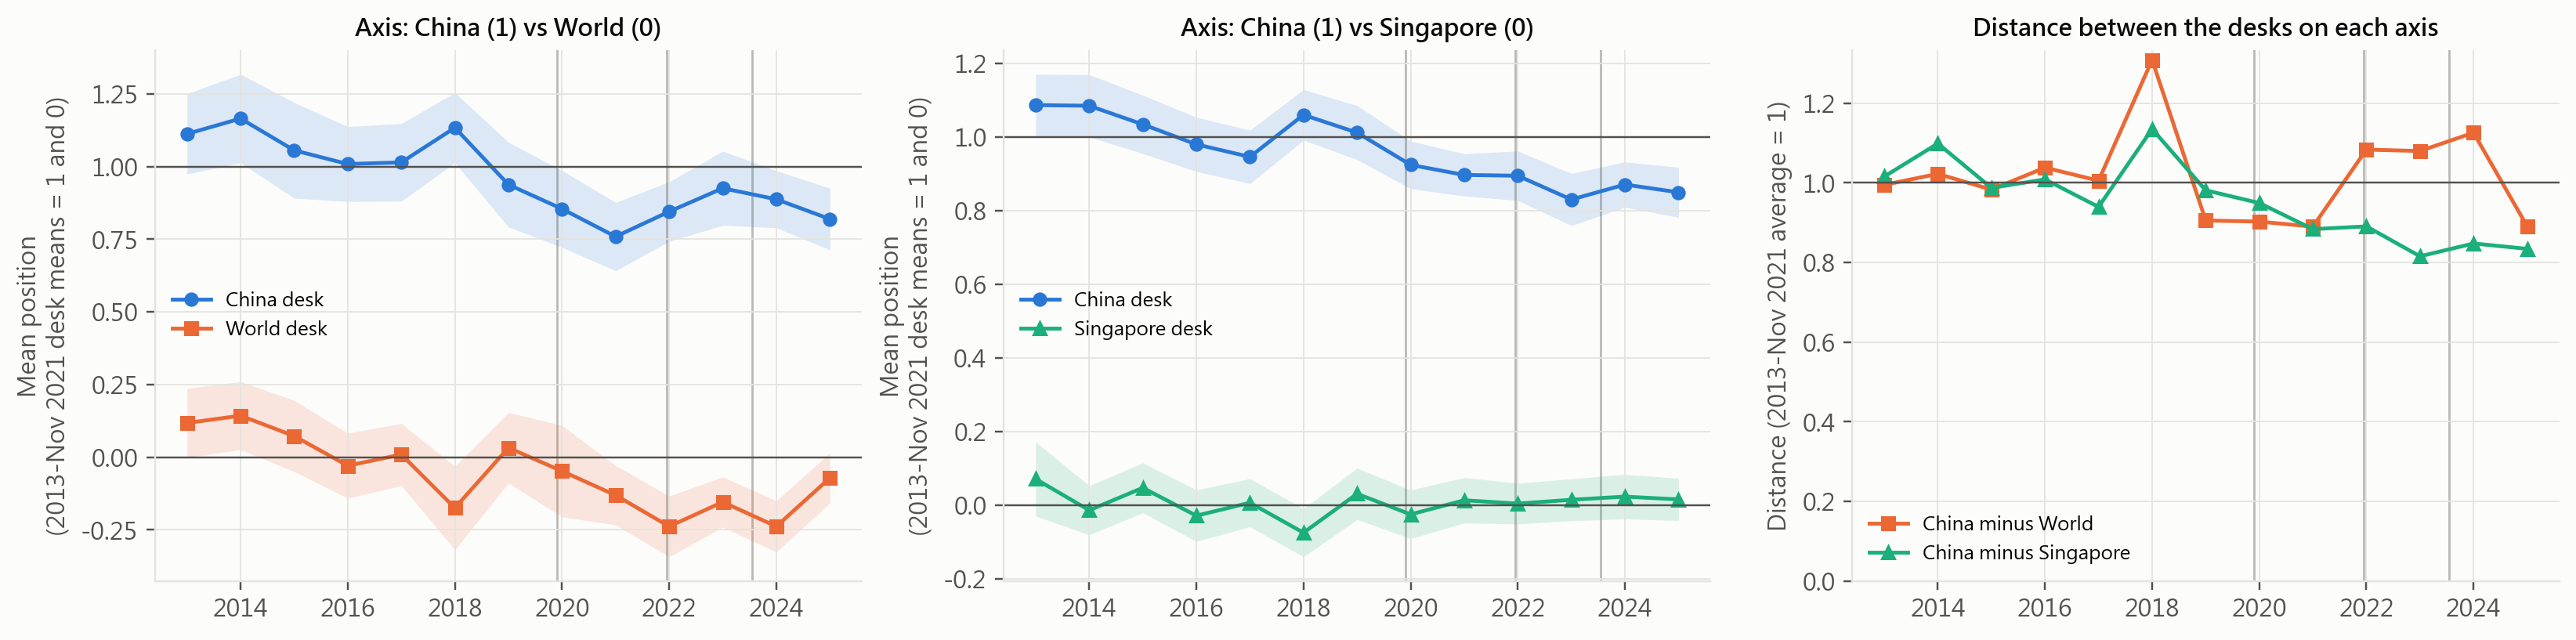
\includegraphics[width=\textwidth]{fig04_which_desk_moved.png}
\caption{Position of each desk's realtime articles on two style axes fixed using articles from before December 2021. On each axis, the pre-2021 averages are 1 for the China desk and 0 for the other desk. The right panel shows the distance between the two desks on each axis (China average minus other desk's average), which is 1 before 2021 on average. Bands are 95\% confidence intervals.}
\label{fig:moved}
\end{figure}

\begin{table}[tbp]
\centering
\small
\setlength{\tabcolsep}{4pt}
\begin{tabular}{@{}llcccc@{}}
\toprule
Axis & Desk & Shift after Dec 2021 & Drift per year & Jump at Dec 2021 [95\% CI] & $q$ \\
\midrule
China vs World & China & $-0.14$ & $-0.036$ & $+0.09$ [$-0.05$, $0.23$] & 0.43 \\
 & World & $-0.18$ & $-0.024$ & $-0.02$ [$-0.16$, $0.12$] & 0.75 \\
 & Distance & $+0.04$ & $-0.014$ & $+0.13$ [$-0.14$, $0.40$] & 0.43 \\
\addlinespace
China vs Singapore & China & $-0.14$ & $-0.018$ & $-0.03$ [$-0.10$, $0.04$] & 0.43 \\
 & Singapore & $+0.01$ & $-0.003$ & $+0.03$ [$-0.03$, $0.10$] & 0.43 \\
 & Distance & $-0.15$ & $-0.014$ & $-0.06$ [$-0.20$, $0.08$] & 0.43 \\
\bottomrule
\end{tabular}
\caption{Which desk moved, realtime corpus. Shift is the average after December 2021 minus the average before, in units of the pre-2021 gap between the desks. Drift is the trend before December 2021, and the jump is the change at December 2021 beyond that trend. Desk rows use article-level models with standard errors clustered by year; distance rows use the 13 yearly values. No jump is significant.}
\label{tab:moved}
\end{table}

\noindent \textbf{Answer to Q1:} No. The realtime China and World desks became somewhat easier to tell apart after 2021, but the change does not survive correction for multiple tests, and on the axis that separated them before 2021 both desks moved together and the distance between them did not change. \textbf{Answer to Q2:} Not at the restructuring. The China desk has moved part of the way toward the Singapore desk in style, but gradually, starting around 2019--2020, and its style also moved toward the World desk's over the same years.

\subsection{Hedging and authority (Q3)}

The World desk hedges most in every corpus and almost every year, and the Singapore desk hedges least (Figure~\ref{fig:levels}). In the realtime corpus, the World desk uses 2.77 hedges per 1,000 words, the China desk 1.64 and the Singapore desk 1.33. In desk leads, the China desk is close to the Southeast Asia desk, with 2.23 and 2.18 hedges per 1,000 words, against 3.31 on the World desk and 1.04 on the Singapore desk.

\begin{figure}[tbp]
\centering
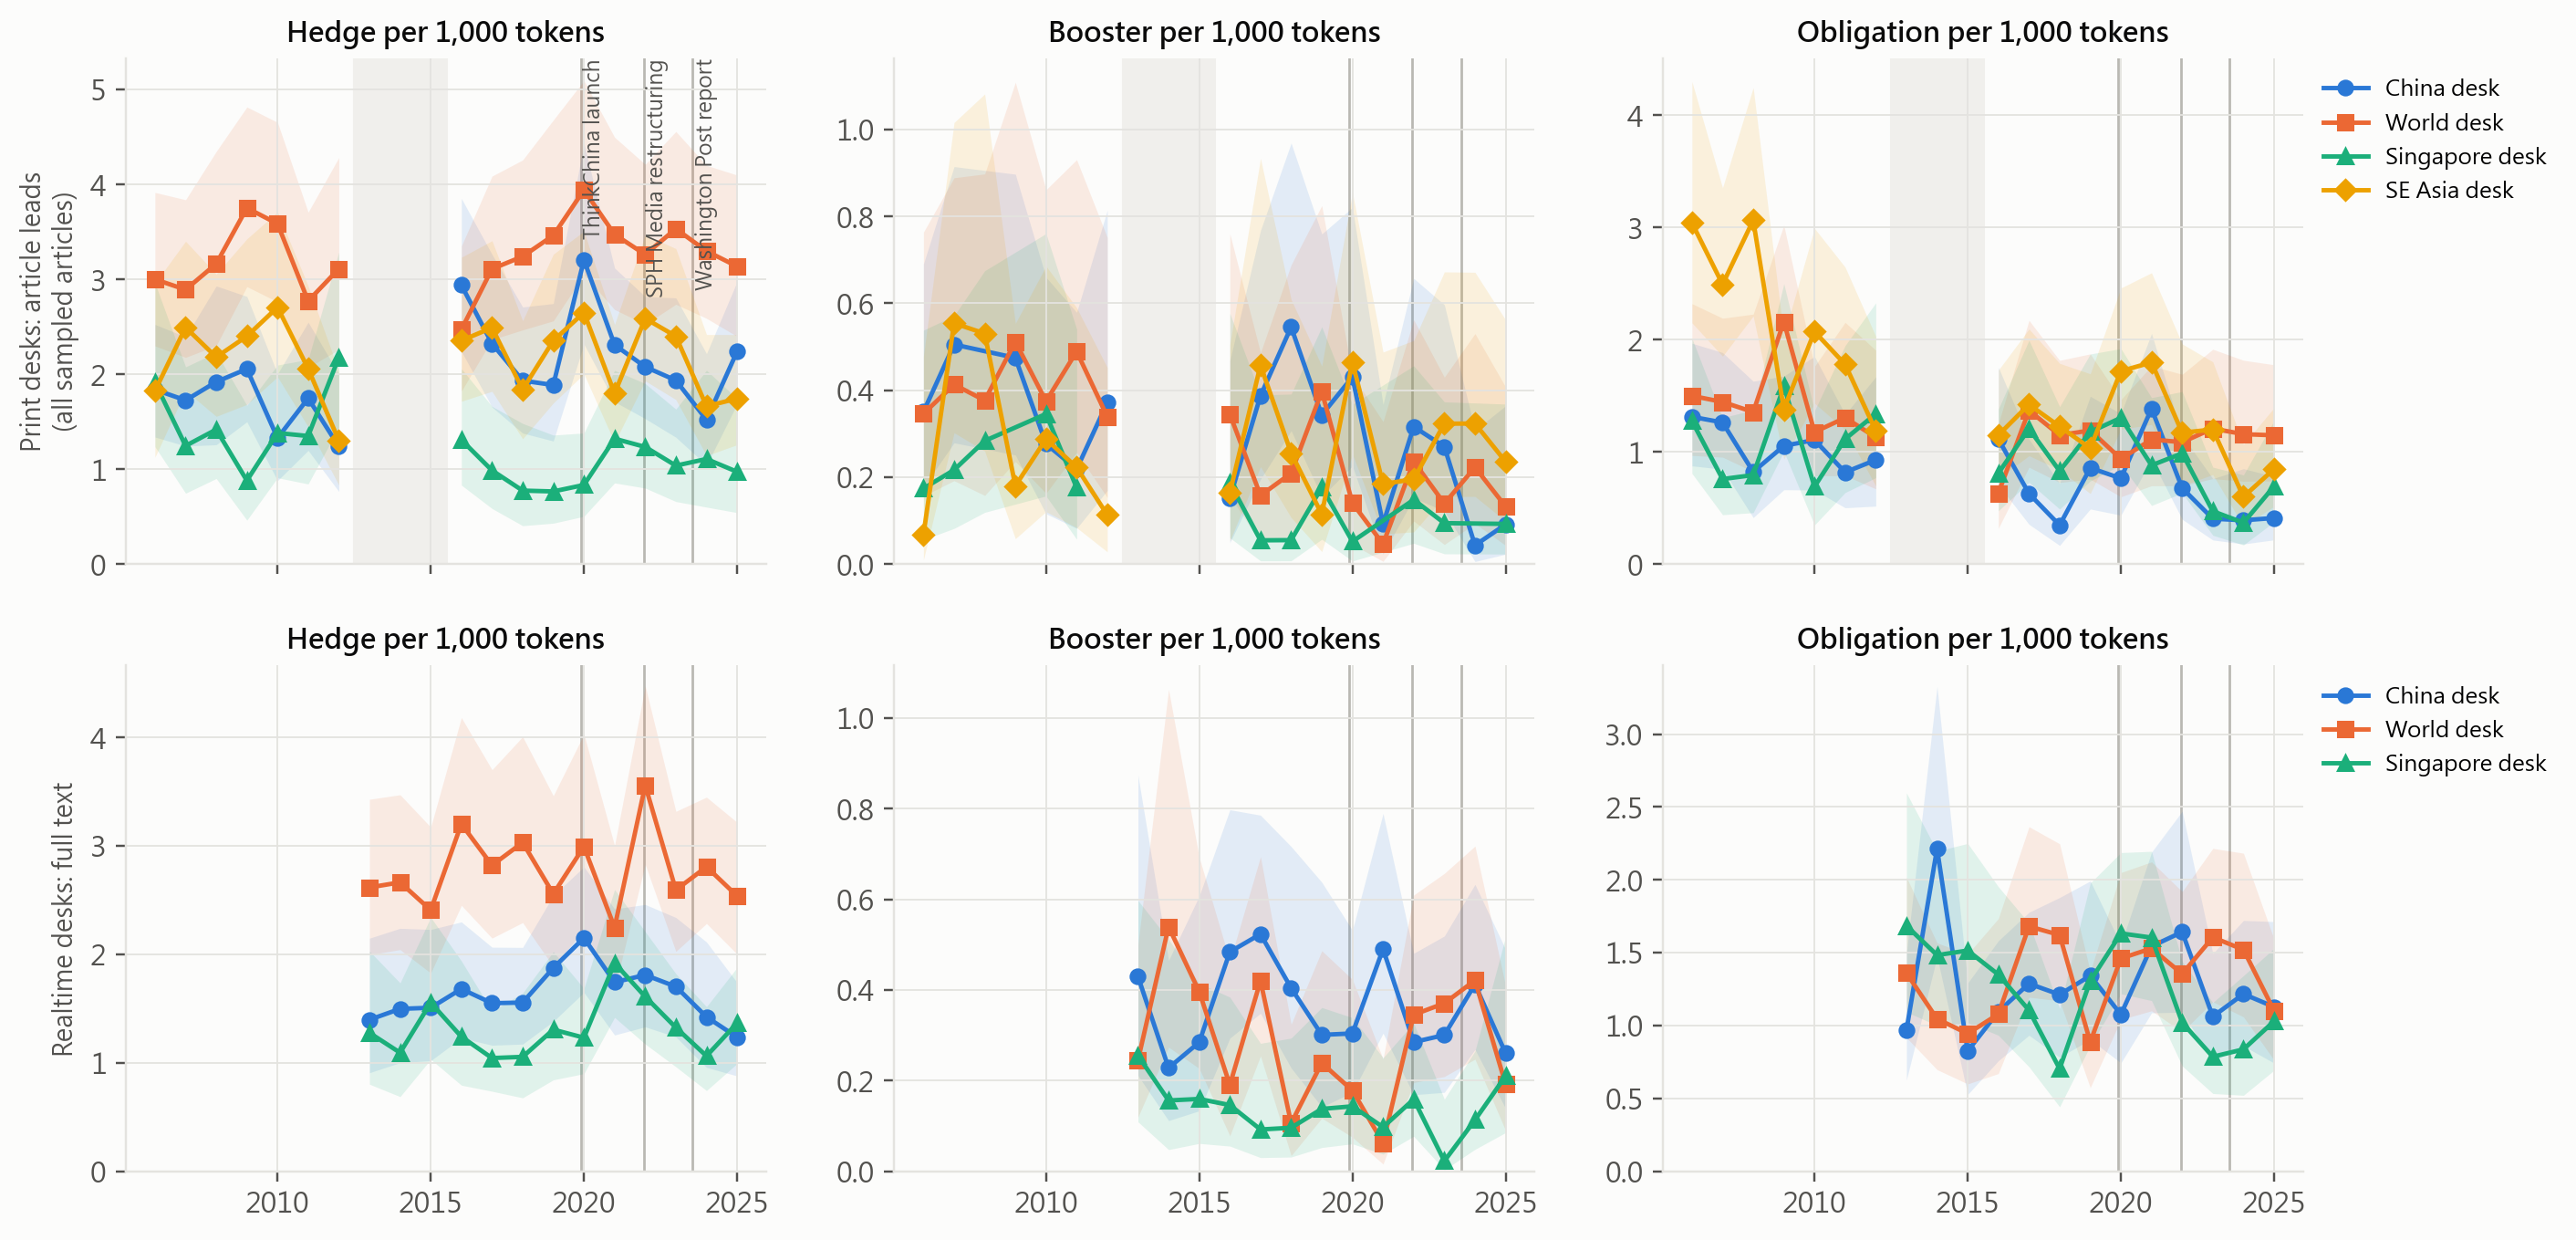
\includegraphics[width=\textwidth]{fig05_marker_rates_by_desk.png}
\caption{Hedges, boosters and obligation words per 1,000 words, by desk and year. The top row uses desk leads for all sampled articles, and the bottom row uses the full text of realtime articles. Bands are 95\% confidence intervals. The grey band marks 2013--2015, when no desk articles were archived.}
\label{fig:levels}
\end{figure}

As rate ratios within the same years (Table~\ref{tab:longrun}), the China desk uses 0.58--0.68 times as many hedges as the World desk in all three corpora, a gap of 32--42\%. But the China desk is not an outlier. Compared with the Singapore desk, it hedges \textit{more} (1.16--2.14 times as often) and attributes far more (1.45--2.51 times). In desk articles, it also uses obligation words less often than the World desk (0.63--0.68). The one category that points toward a more assertive China desk is boosters: in the realtime corpus, it uses them 1.26 times as often as the World desk, though this is not significant after correction ($q = 0.08$). This pattern fits the literature on journalism in Singapore, which describes domestic reporting as cooperative with authority and focused on nation-building rather than on a watchdog role \cite{massey,hanitzsch,wong}. By these measures, the desk that hedges least is the Singapore desk, not the China desk.

\begin{table}[tbp]
\centering
\small
\begin{tabular}{@{}llccccc@{}}
\toprule
Corpus & vs & Hedge & Booster & Obligation & Permission & Attribution \\
\midrule
Desk, 2006--12 & World & \textbf{0.60} & 1.20 & \textbf{0.68} & 1.07 & \textbf{0.80} \\
 & Singapore & \textbf{1.16} & \textbf{2.32} & \textbf{0.83} & 0.93 & \textbf{1.45} \\
 & SE Asia & \textbf{0.82} & \textbf{1.26} & \textbf{0.49} & \textbf{0.79} & \textbf{0.75} \\
\addlinespace
Desk leads, 2016--25 & World & \textbf{0.68} & 1.33 & \textbf{0.63} & 0.90 & \textbf{1.16} \\
 & Singapore & \textbf{2.14} & \textbf{3.15} & 0.80 & 0.87 & \textbf{2.51} \\
 & SE Asia & 1.02 & 0.95 & \textbf{0.57} & \textbf{0.75} & \textbf{1.19} \\
\addlinespace
Realtime, 2013--25 & World & \textbf{0.58} & 1.26 & 0.95 & \textbf{0.71} & \textbf{0.86} \\
 & Singapore & \textbf{1.23} & \textbf{2.74} & 1.08 & 0.91 & \textbf{2.19} \\
\bottomrule
\end{tabular}
\caption{China-desk rate ratios against each comparison desk, with year fixed effects. Values below 1 mean the China desk uses the markers less often. Bold values are significant after false discovery rate correction ($q < 0.05$).}
\label{tab:longrun}
\end{table}

\paragraph{Voice or topic?} The hedging gap is not simply a matter of what the two desks cover (Table~\ref{tab:topic}). Comparing articles on the same topic shrinks the realtime China/World hedging ratio from 0.58 to between 0.67 and 0.78, depending on the number of topics, and the legacy ratio from 0.60 to 0.66. Topic composition therefore accounts for between a fifth and a half of the gap (measured on the log scale). The rest is a difference in how the desks write: on the same subjects, the China desk hedges a fifth to a third less. The same holds when only topics that both desks cover are compared (0.67 and 0.66). Holding topic fixed also changes the obligation result: on the same topics, the China desk uses \textit{fewer} obligation words than the World desk in both corpora (0.69--0.77), the opposite of the authority hypothesis. Boosters move the other way in the realtime corpus (1.26--1.47 times the World desk's rate, significant in two of the three versions), but not in the legacy corpus (1.10--1.17), so I treat this as weak evidence that the China desk states things with more certainty.

\begin{table}[tbp]
\centering
\small
\begin{tabular}{@{}lcccc@{}}
\toprule
 & Year FE only & + 20 topics & + 40 topics & Shared topics only \\
\midrule
\multicolumn{5}{@{}l}{\textit{Realtime, 2013--25}} \\
Hedge & 0.58 [0.52, 0.66] & 0.78 [0.67, 0.90] & 0.67 [0.58, 0.77] & 0.67 [0.58, 0.78] \\
Booster & 1.26 [0.99, 1.61] & 1.39 [1.04, 1.84] & 1.26 [0.96, 1.67] & 1.47 [1.04, 2.08] \\
Obligation & 0.95 [0.82, 1.11] & 0.75 [0.63, 0.90] & 0.77 [0.63, 0.94] & 0.74 [0.60, 0.93] \\
\addlinespace
\multicolumn{5}{@{}l}{\textit{Desk, 2006--12}} \\
Hedge & 0.60 [0.55, 0.66] & 0.66 [0.59, 0.75] & 0.66 [0.59, 0.74] & 0.66 [0.58, 0.75] \\
Booster & 1.20 [0.99, 1.44] & 1.17 [0.89, 1.52] & 1.11 [0.85, 1.44] & 1.10 [0.83, 1.45] \\
Obligation & 0.68 [0.60, 0.76] & 0.69 [0.58, 0.83] & 0.72 [0.62, 0.83] & 0.70 [0.60, 0.83] \\
\bottomrule
\end{tabular}
\caption{China/World rate ratios [95\% CI] with and without topic fixed effects (NMF topics, full texts). ``Shared topics'' keeps only the 40-topic clusters in which each desk supplies at least 20\% of the articles. Permission and attribution are not shown.}
\label{tab:topic}
\end{table}

The gap against the World desk is steady over time (Figure~\ref{fig:irr}). The hedging ratio is below 1 in almost every year from 2006 to 2025, in both corpora, and it does not change at 2021.

\begin{figure}[tbp]
\centering
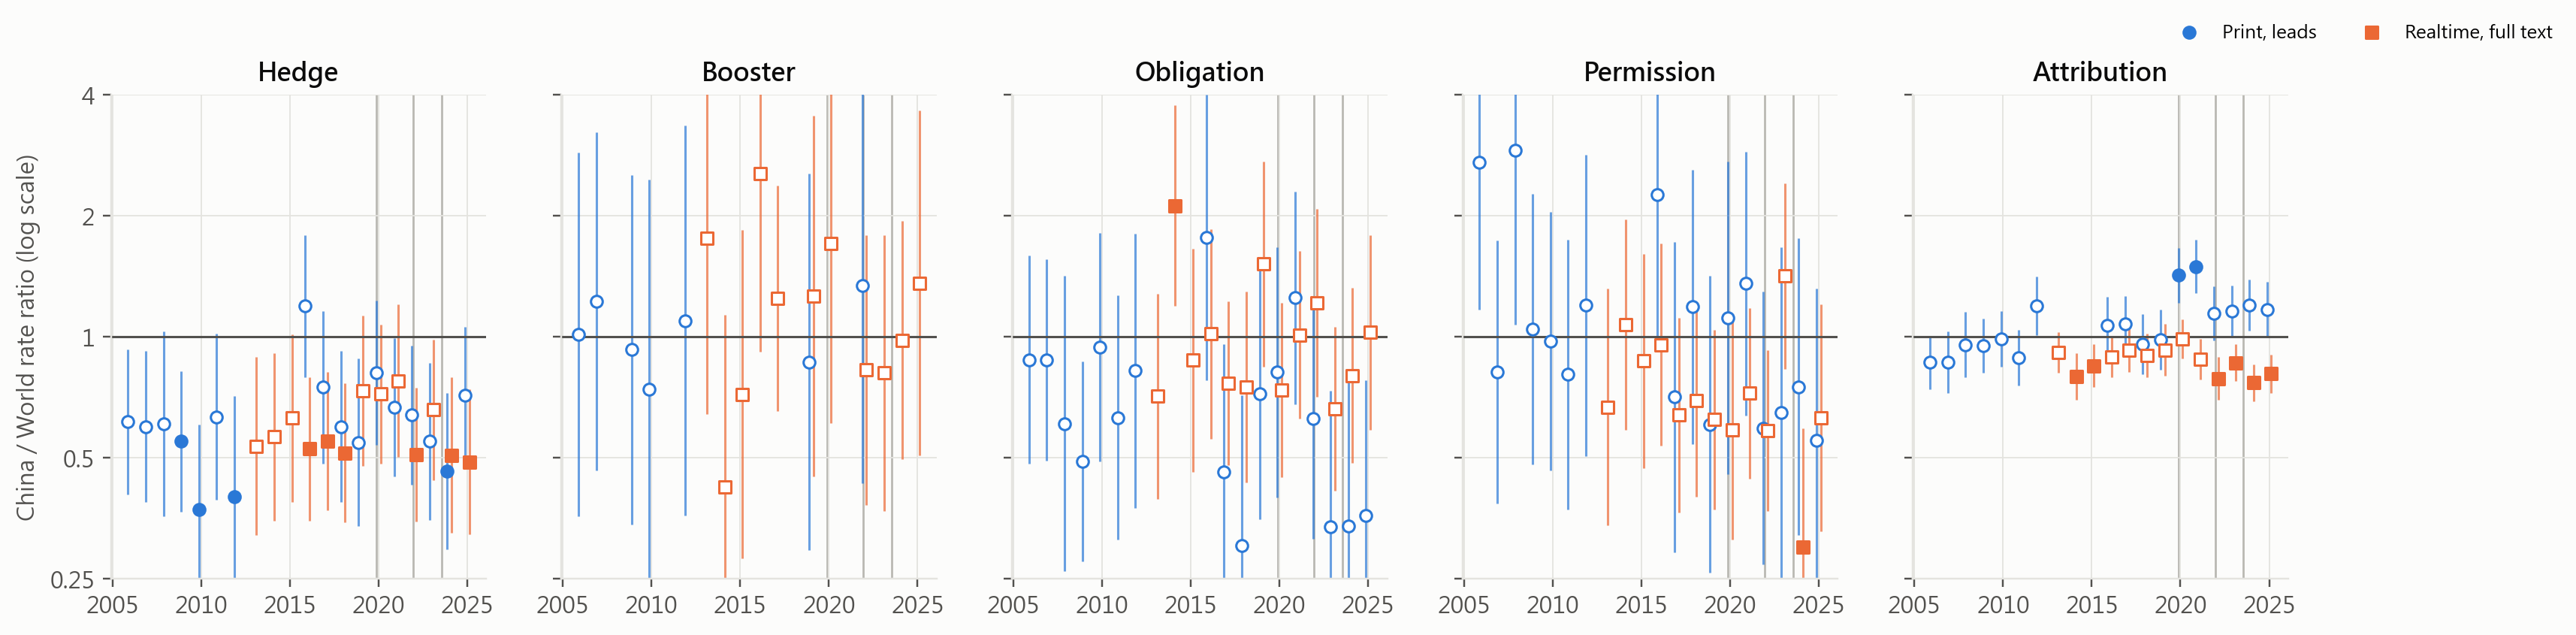
\includegraphics[width=\textwidth]{fig06_china_world_rate_ratios.png}
\caption{China/World rate ratio by year, on a log scale. Blue points are desk leads and orange points are realtime full texts. Filled markers are significant after false discovery rate correction, and hollow markers are not. Vertical lines mark the three events.}
\label{fig:irr}
\end{figure}

The difference-in-differences tests confirm this (Table~\ref{tab:did}). In the realtime corpus, no category changes significantly after correction, at either level. The hedging ratio after the restructuring is 0.91 times its earlier value (95\% CI 0.71--1.17), so a fall of more than about 30\% relative to the World desk can be ruled out. Attribution fell by about 8\% relative to the World desk ($q = 0.056$ at the article level, $0.068$ at the year level), but there are two simpler explanations. When the break is moved to other years, the estimate declines smoothly (Figure~\ref{fig:placebo}): it is 0.995 for a break in 2014, 0.95 for 2019, 0.92 for 2021 and 0.89 for 2023, which is the pattern of a trend rather than a break. And once topics are held fixed, the change disappears (0.97, 95\% CI 0.90--1.03). In desk leads, one article-level test survives correction: obligation words fell to 0.53 times their earlier ratio to the World desk ($q = 0.044$). This is the opposite of what the hypothesis predicts, and it is not robust. At the year level, it is not significant ($q = 0.14$), and the placebo estimates for desk leads vary widely from year to year (0.43 to 1.02), so December 2021 does not stand out. Negative binomial models give estimates within 0.03 of the Poisson ones; they estimate the attribution decline more precisely ($p = 0.001$), but it remains a trend, not a break.

\begin{table}[tbp]
\centering
\small
\begin{tabular}{@{}lcccc@{}}
\toprule
 & \multicolumn{2}{c}{Article level} & \multicolumn{2}{c}{Year level} \\
\cmidrule(lr){2-3}\cmidrule(lr){4-5}
Category & Change [95\% CI] & $q$ & Change [95\% CI] & $q$ \\
\midrule
\multicolumn{5}{@{}l}{\textit{Realtime, full text (2013--2025)}} \\
Hedge & 0.91 [0.71, 1.17] & 0.60 & 0.88 [0.72, 1.08] & 0.48 \\
Booster & 0.62 [0.38, 1.02] & 0.15 & 0.81 [0.45, 1.46] & 0.64 \\
Obligation & 1.01 [0.72, 1.41] & 0.97 & 0.92 [0.60, 1.39] & 0.64 \\
Permission & 0.89 [0.64, 1.23] & 0.60 & 0.85 [0.32, 2.26] & 0.64 \\
Attribution & 0.92 [0.86, 0.98] & 0.056 & 0.90 [0.84, 0.97] & 0.068 \\
\addlinespace
\multicolumn{5}{@{}l}{\textit{Desk leads (2016--2025)}} \\
Hedge & 0.83 [0.63, 1.09] & 0.29 & 0.79 [0.56, 1.12] & 0.21 \\
Booster & 0.61 [0.26, 1.43] & 0.32 & -- & -- \\
Obligation & 0.53 [0.33, 0.85] & 0.044 & 0.53 [0.26, 1.08] & 0.14 \\
Permission & 0.55 [0.32, 0.95] & 0.076 & 0.58 [0.35, 0.95] & 0.14 \\
Attribution & 1.00 [0.91, 1.11] & 0.94 & 1.02 [0.83, 1.24] & 0.86 \\
\bottomrule
\end{tabular}
\caption{Difference-in-differences estimates of the change in the China/World rate ratio after 1 December 2021. A value of 1 means no change. Article level: Poisson model with desk and year fixed effects. Year level: Welch test on yearly log rate ratios. Boosters in leads are too rare for yearly ratios (fewer than five per desk in most years).}
\label{tab:did}
\end{table}

\begin{figure}[tbp]
\centering
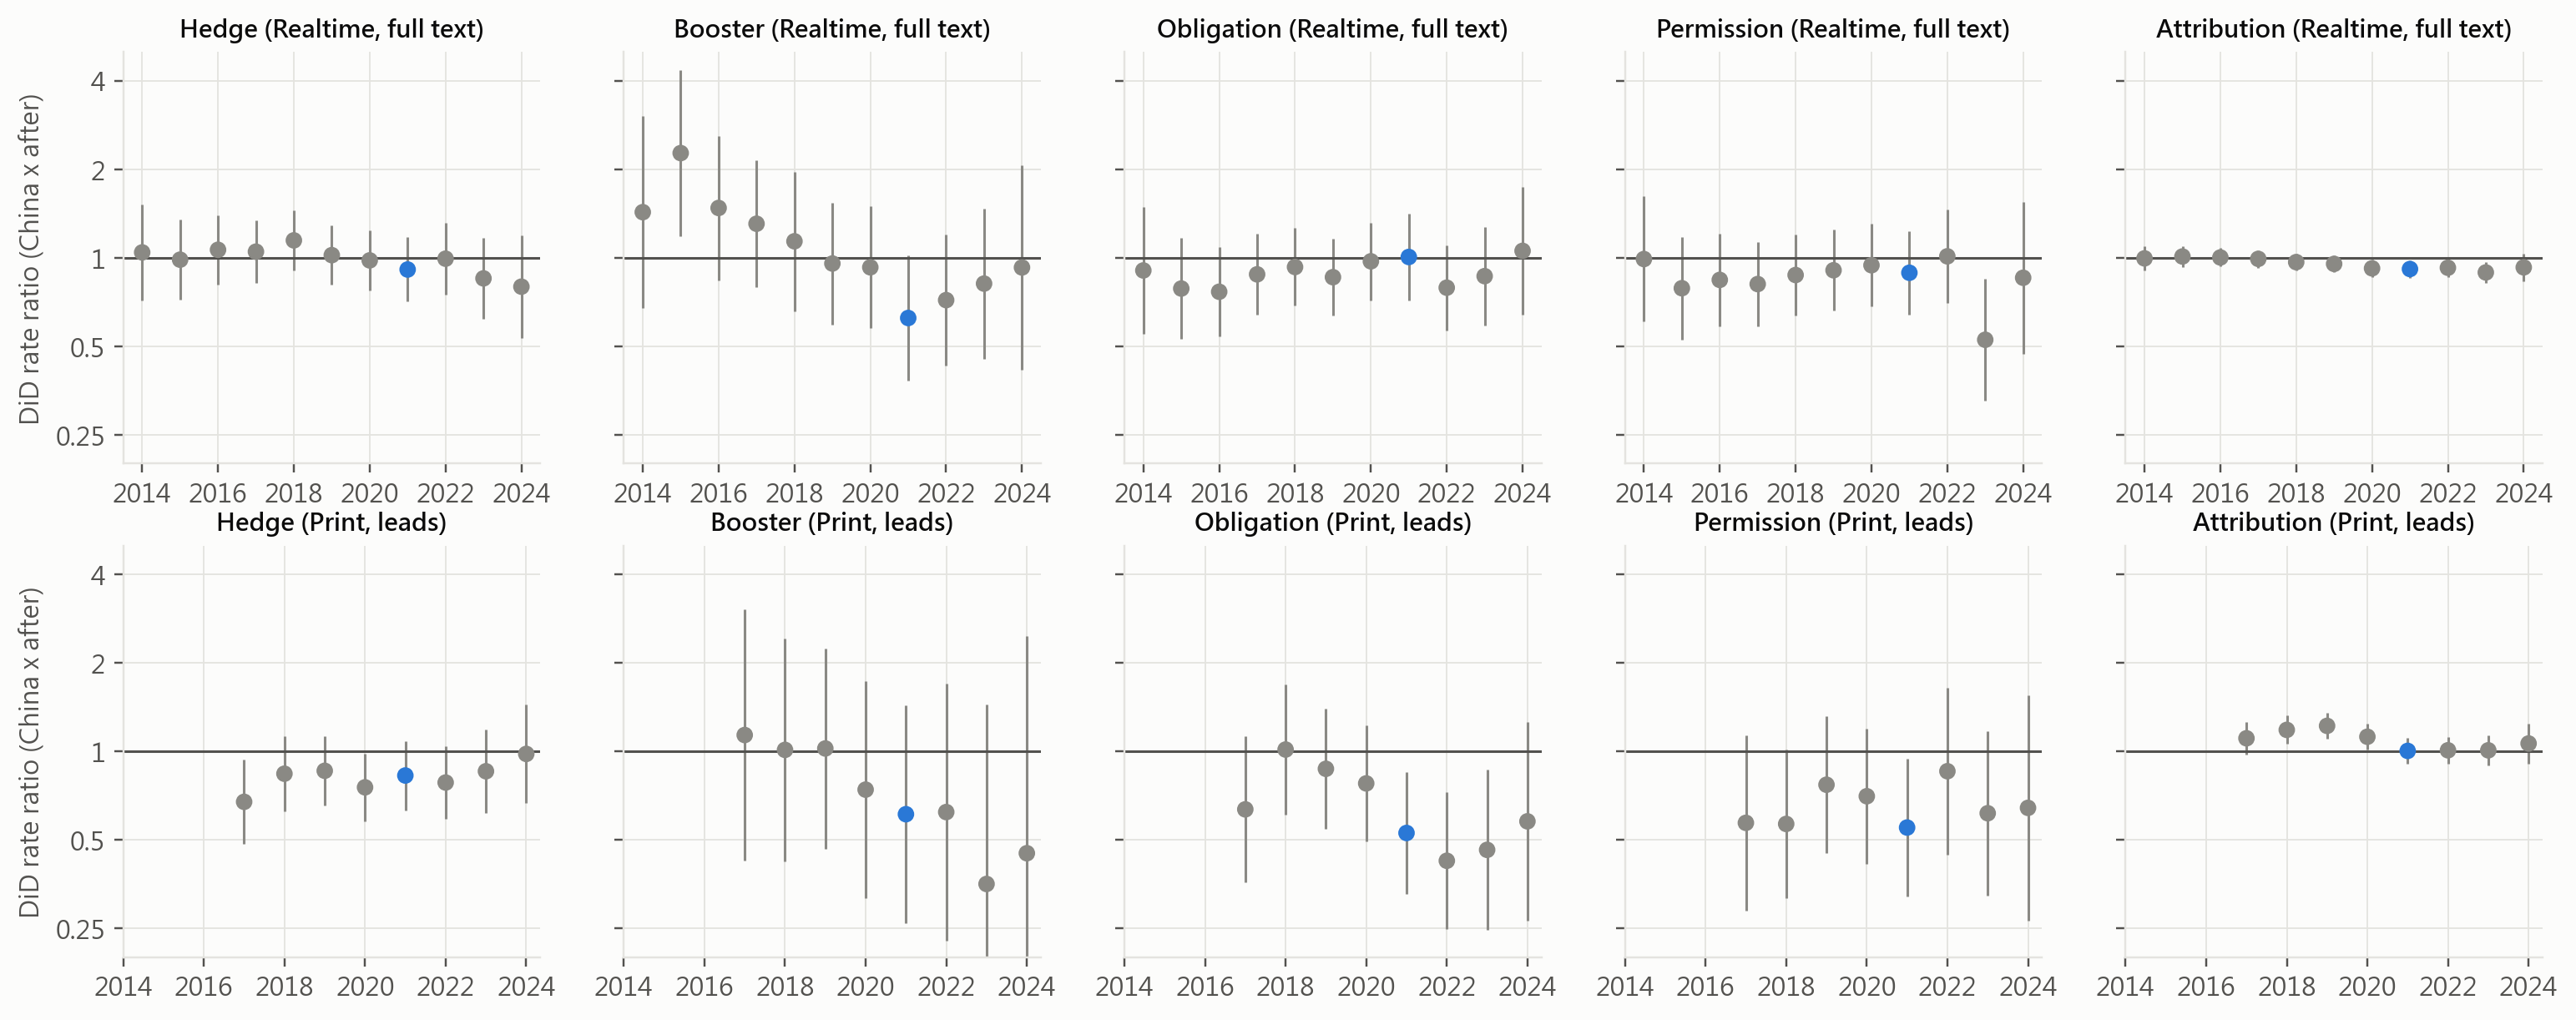
\includegraphics[width=\textwidth]{fig07_placebo_breaks.png}
\caption{Difference-in-differences estimates with the break moved to 1 December of each year. Blue is the real restructuring date and grey points are placebo dates. The top row uses the realtime corpus and the bottom row desk leads.}
\label{fig:placebo}
\end{figure}

The choice of control desk matters for one category. Against the Singapore desk instead of the World desk, the China desk's realtime obligation rate rose after 2021 (1.53, 95\% CI 1.09--2.15; year level $p = 0.03$), which is the direction the hypothesis predicts. Against the World and Singapore desks pooled, the change is smaller and not significant (1.20, 95\% CI 0.90--1.61). The hedging results do not depend on the control desk (0.91--0.93).

Changes in individual words can cancel out within a category, so I also compare each word separately (Figure~\ref{fig:terms}). The hedging gap is almost entirely one word: 可能 (\textit{keneng}, ``possibly'') accounts for 84\% of the realtime China--World gap and 79\% of the legacy gap, and its China/World ratio is 0.51--0.56 in every period; 可能性 (\textit{kenengxing}, ``possibility'') and 估計 (\textit{guji}, ``estimate'') account for most of the rest. Two words show large changes in their ratio after December 2021, and both need a closer look. 據 (\textit{ju}, ``according to'') goes from 1.36 to 2.72 times the World desk's rate, but not because the China desk uses it more: its rate on the China desk fell from 36.7 to 26.8 per 10,000 words, while on the World desk it fell much further, from 27.0 to 9.9. 不得 (\textit{bude}, ``must not'') rises from 1.75 to 9.95 times the World desk's rate, and here the China desk's own rate tripled (1.0 to 3.0 per 10,000 words). In a random sample of these uses, 不得 appears almost always inside quoted rules: regulations, court orders, bail conditions and official statements on Taiwan. That fits the sourcing change described next, but it rests on only 29 China-desk articles after 2021. Most other words are too rare to change significantly.

\begin{figure}[tbp]
\centering
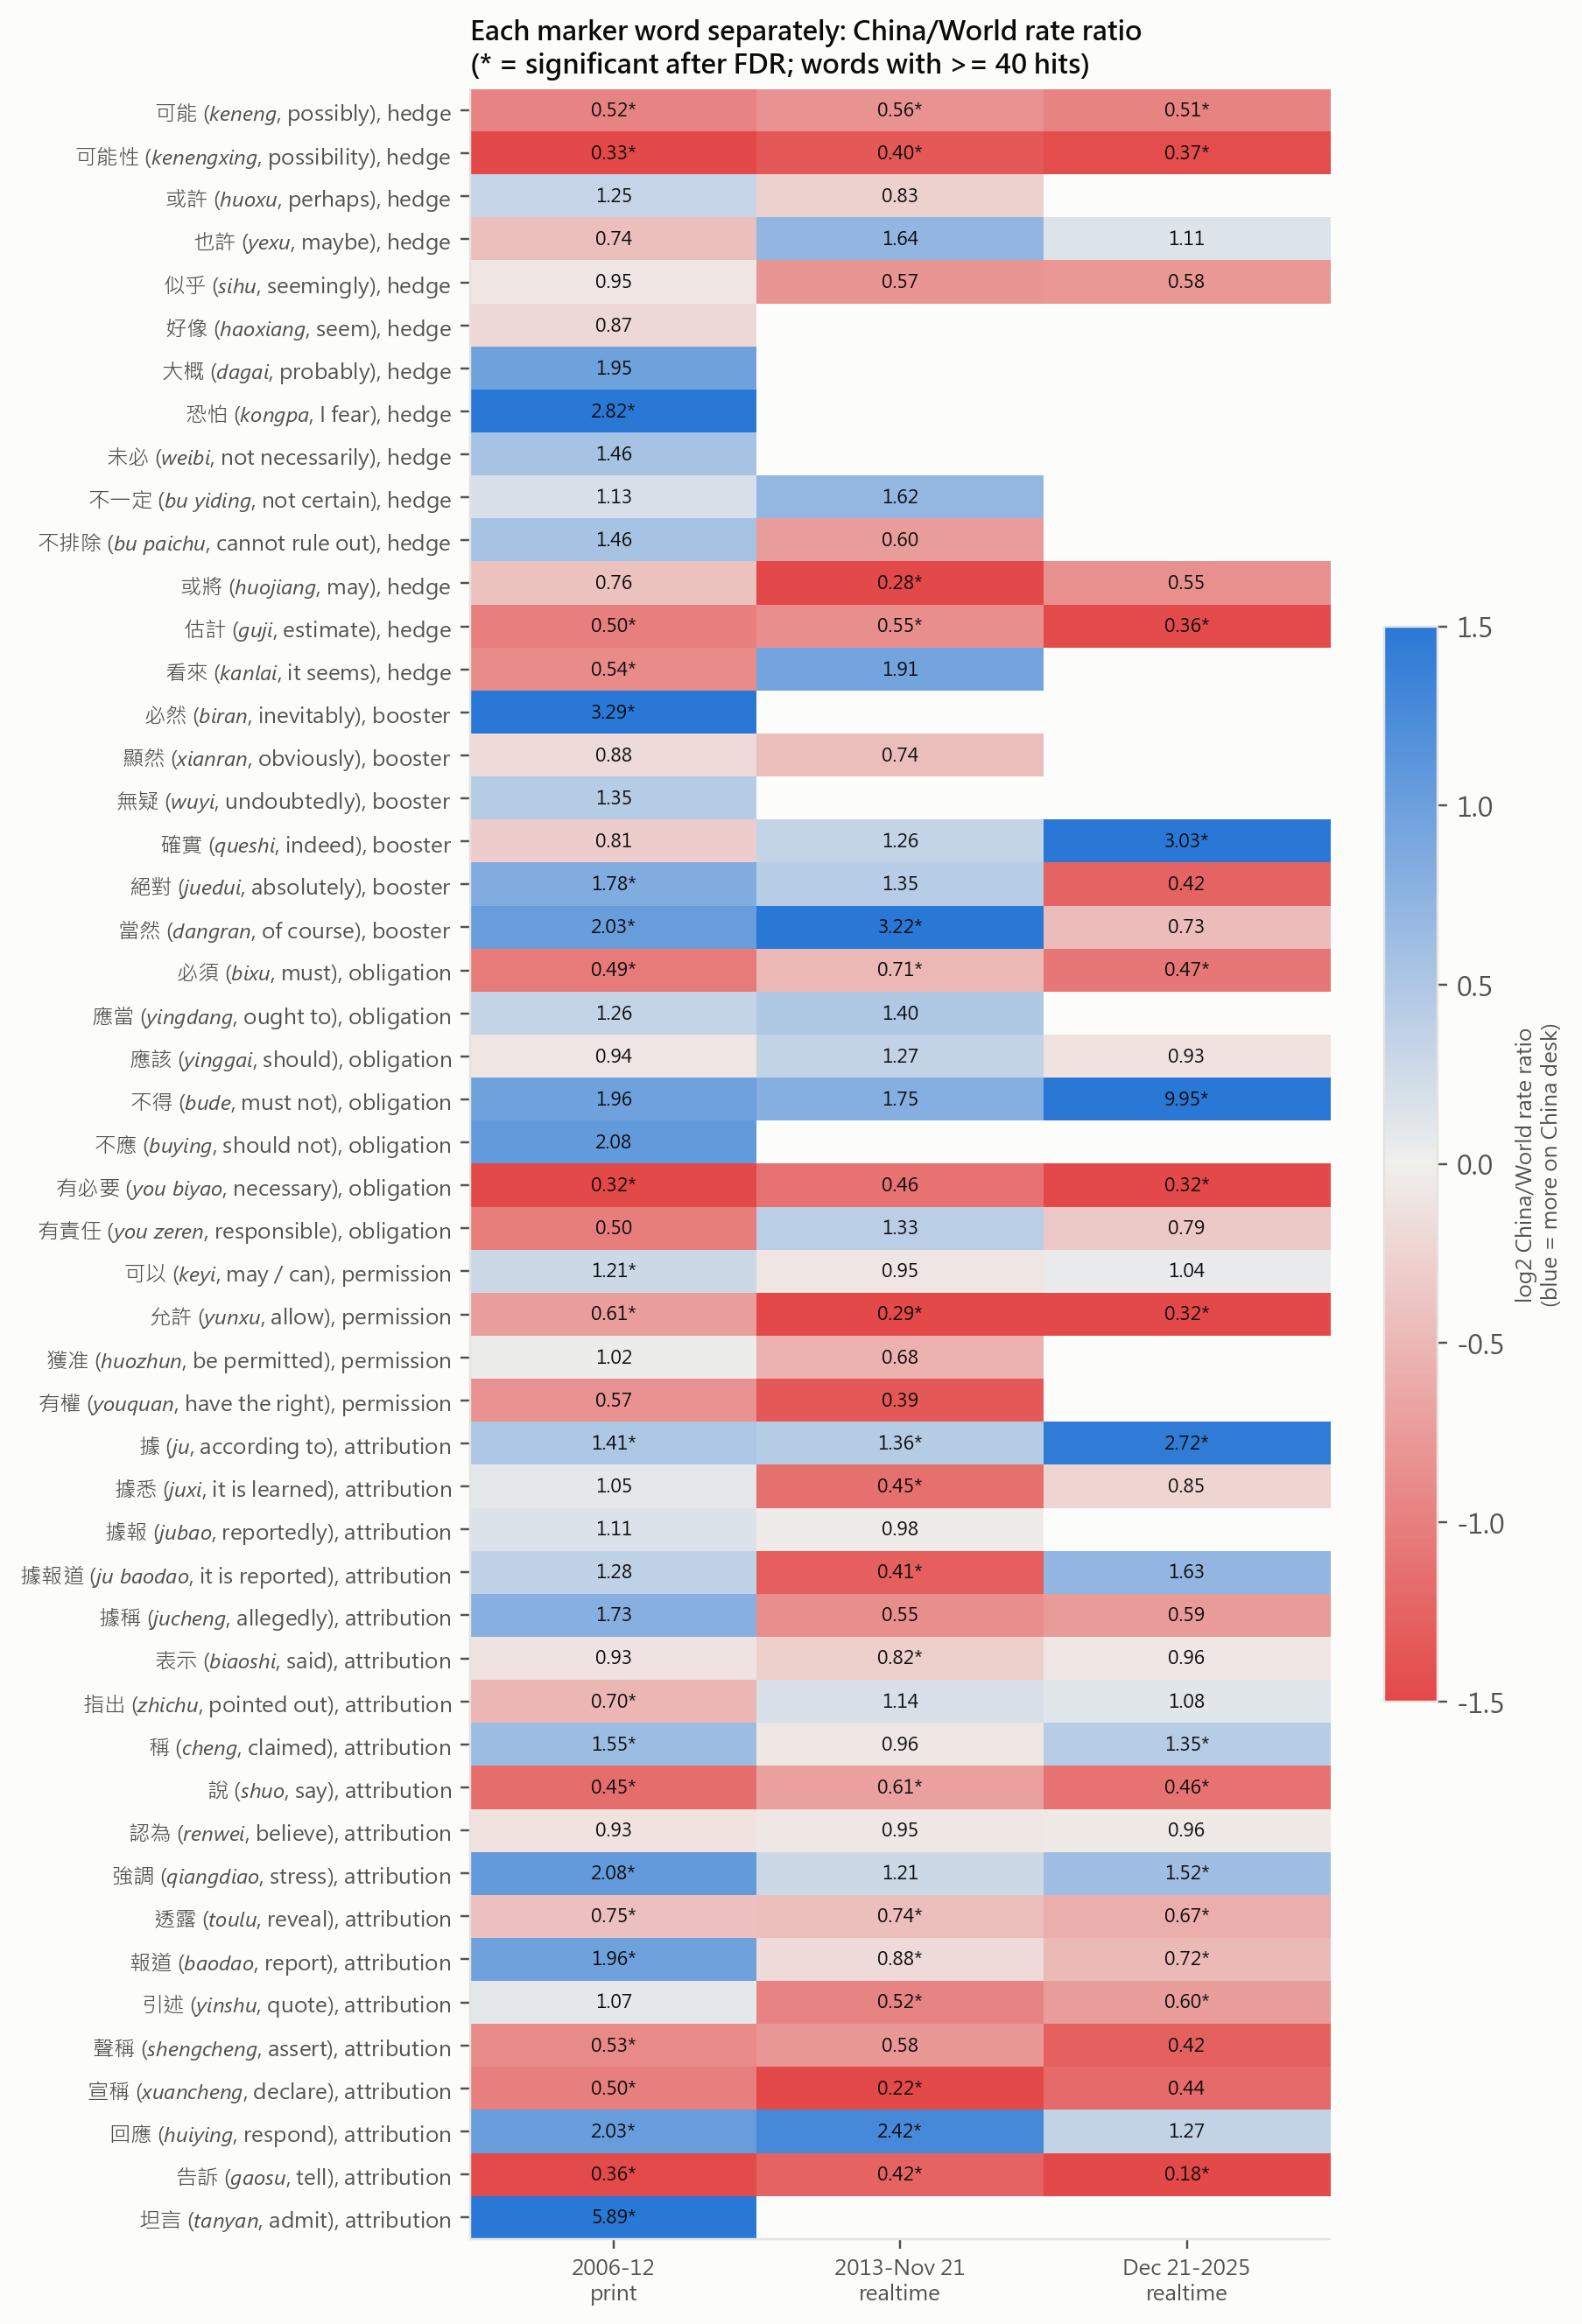
\includegraphics[height=0.8\textheight]{fig08_per_word_rate_ratios.png}
\caption{China/World rate ratio for each marker word in three periods, namely desk articles from 2006 to 2012 and realtime articles before and after December 2021. Blue means the China desk uses the word more often. An asterisk marks ratios that are significant after false discovery rate correction. Words with fewer than 40 occurrences are omitted.}
\label{fig:terms}
\end{figure}

\noindent \textbf{Answer to Q3:} Partly, but not in the way the hypothesis states, and not as a change. The China desk does hedge much less than the World desk, a fifth to a third less even on the same topics, but this has been true for twenty years and it hedges more than the Singapore desk. It does not use more obligation language than the World desk; on the same topics, it uses less. Nothing in its epistemic stance changed at the restructuring.

\subsection{What the desks write about}

The words that best separate the China and World desks are mostly about geography (Figure~\ref{fig:words}), with 中國 (China), 台灣 (Taiwan), 香港 (Hong Kong) and 兩岸 (\textit{liang'an}, ``cross-Strait'') on one side and 美國 (United States), 俄羅斯 (Russia) and 烏克蘭 (Ukraine) on the other. The largest changes after 2021 are shared by both desks and come from house style. Zaobao began to give dates as weekdays (星期一 \textit{xingqiyi} to 星期天 \textit{xingqitian}, ``Monday'' to ``Sunday'') instead of 今天 (\textit{jintian}, ``today'') and 昨天 (\textit{zuotian}, ``yesterday''), dropped the dateline 聯合早報網訊 (``Lianhe Zaobao online report'') and used 表示 (\textit{biaoshi}, ``said'') less often. This is why the World desk is needed as a control. A study of the China desk alone would have mistaken these changes for a change in how the desk writes.

\begin{figure}[tbp]
\centering
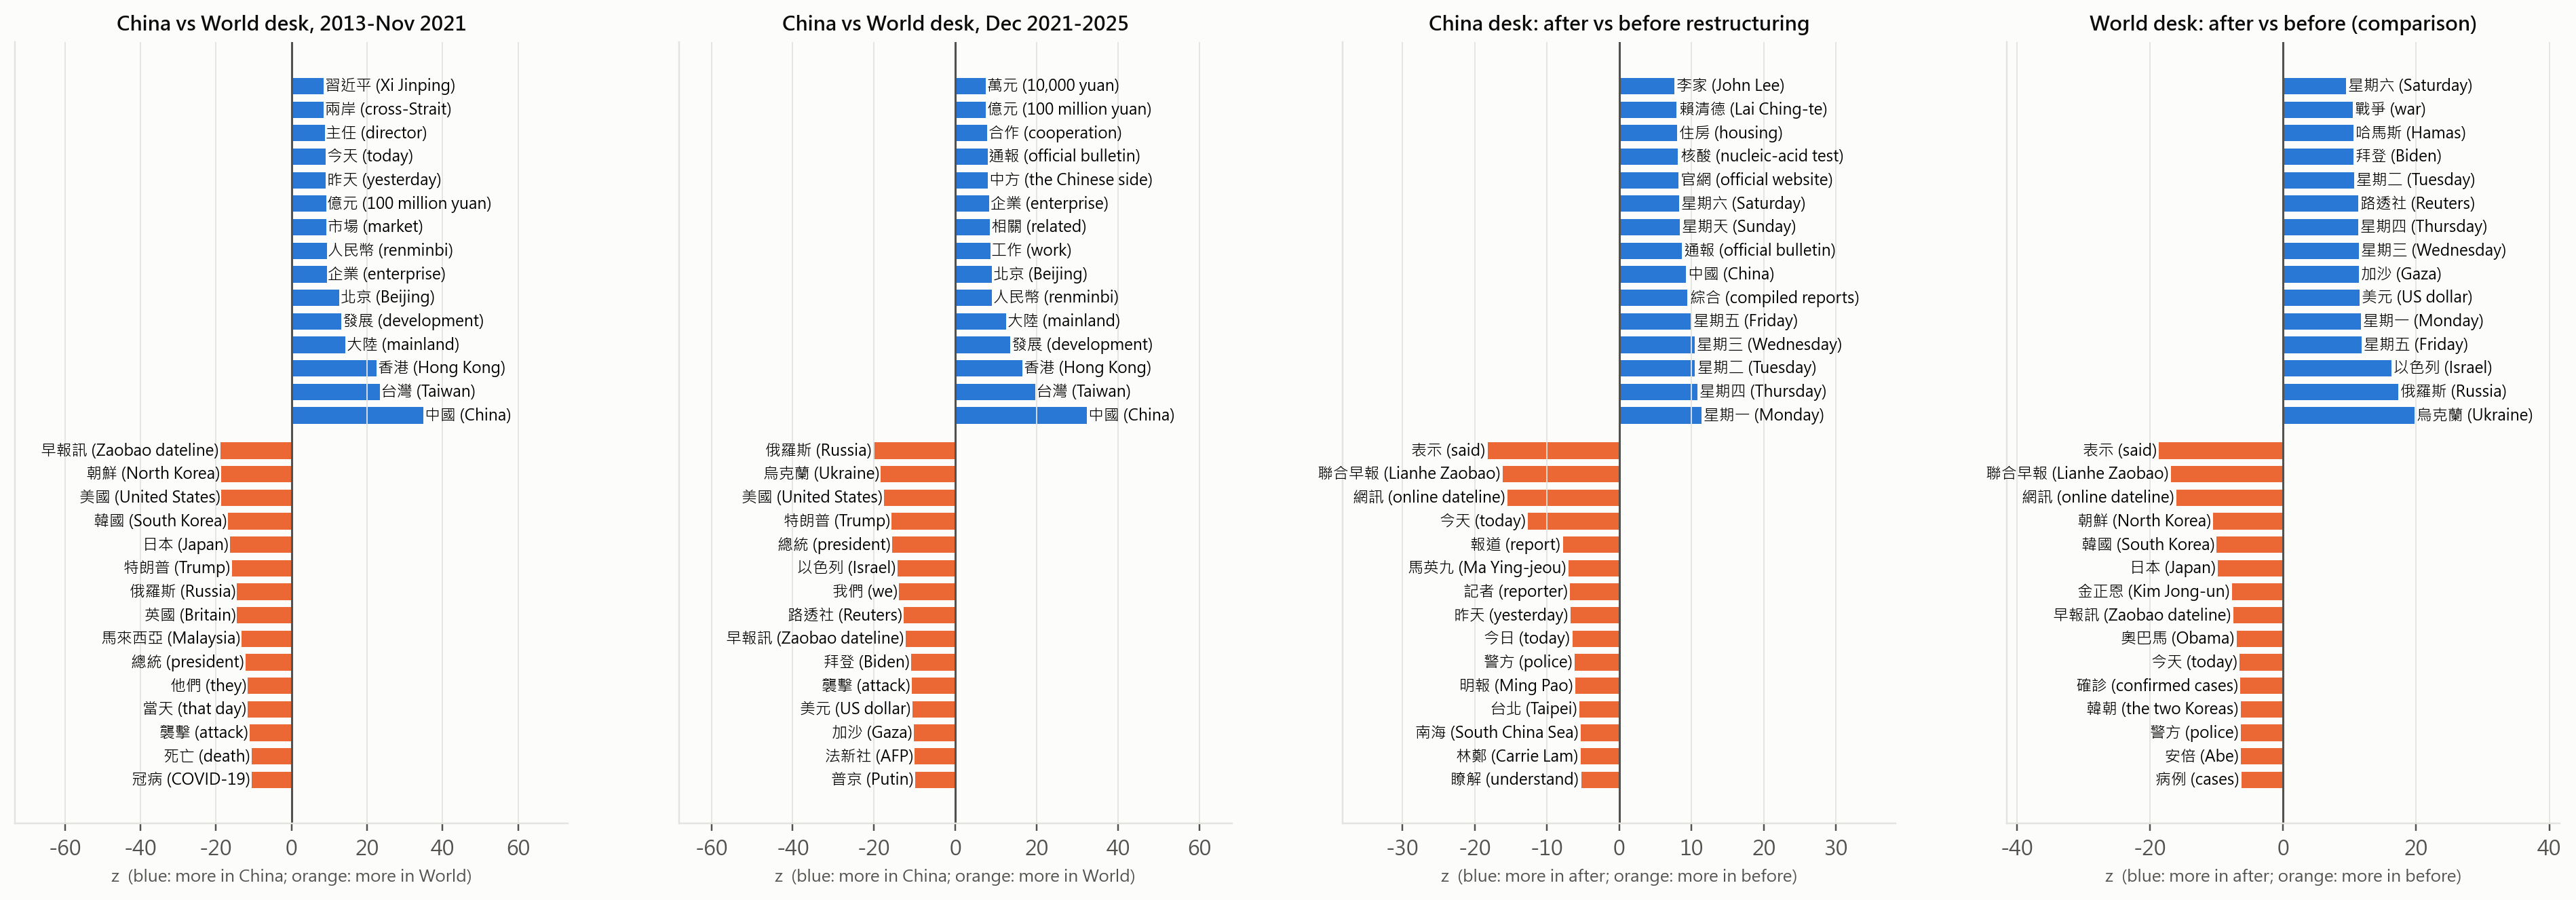
\includegraphics[width=\textwidth]{fig09_distinctive_words.png}
\caption{The most distinctive words in the realtime corpus (weighted log-odds with an informative Dirichlet prior). From left to right, the panels compare China with World before December 2021, China with World after, the China desk after with before, and the World desk after with before. English glosses are in brackets; 李家 is the segmenter's split of 李家超 (John Lee).}
\label{fig:words}
\end{figure}

After removing the changes the two desks share, the words that rose specifically on the China desk include COVID-control terms (隔離 \textit{geli} ``quarantine'', 核酸 \textit{hesuan} ``nucleic-acid test'', 檢測 \textit{jiance} ``testing'', 防疫 \textit{fangyi} ``epidemic control''), the economy (經濟 \textit{jingji}, 住房 \textit{zhufang} ``housing'', 關稅 \textit{guanshui} ``tariffs''), new leaders (賴清德, Lai Ching-te, in Taiwan; 李家超, John Lee, in Hong Kong) and two words about sources, 通報 (``official bulletin'') and 官網 (``official website''). The words that fell include 記者 (\textit{jizhe}, ``reporter''), 中央社 (Taiwan's Central News Agency), 明報 (Hong Kong's \textit{Ming Pao}), 遊行 (\textit{youxing}, ``protest march'') and 林鄭 (Carrie Lam). These lists are descriptive rather than tests, so I followed them up with a direct count of sources.

\subsection{Sources (exploratory)}
\label{sec:sources}

Two trends stand out. First, references to official channels on the China desk rose steadily (Figure~\ref{fig:sources}), from 1.0 per 10,000 characters in 2013 to 3.4 in 2021 and 9.2 in 2024, while the World desk stayed between 0.2 and 2.9, with its highest values in the pandemic years 2020--2021. Relative to the World desk, these references rose about threefold after December 2021 (rate ratio 3.33, 95\% CI 2.09--5.30, $q < 0.001$), and December 2021 gives the largest estimate of all eleven possible break years (the others range from 1.5 to 3.2). In a random sample of these mentions, most are police statements, notices from the Central Commission for Discipline Inspection, ministry and local-government websites and regulators, and a smaller number are company websites.

The increase is not explained by pandemic coverage. Only 15\% of China-desk articles after the restructuring mention COVID, and dropping every article that does leaves the estimate unchanged (3.66, 95\% CI 2.09--6.44). Dropping the years 2020--2022 entirely, so that 2013--2019 is compared directly with 2023--2025, makes it larger (5.10, 95\% CI 2.44--10.67), because the China desk's rate kept rising after the pandemic controls ended. The change also holds at the level of years, which allows for desk-specific news shocks (4.09, 95\% CI 1.32--12.70, $p = 0.02$).

Second, citations of Chinese state media did not rise (Table~\ref{tab:shares}). Their average share of all named media citations on the China desk fell from 33\% in 2013--2018 to 21--22\% from 2019 on. The share of international wires and media rose from 13\% to 30--31\%, and the share of Hong Kong media fell from 25\% to 15\% after 2021. None of these changes in share is a significant break after correction, so they are better described as trends, and each rests on only 150--230 named citations a year.

\begin{figure}[tbp]
\centering
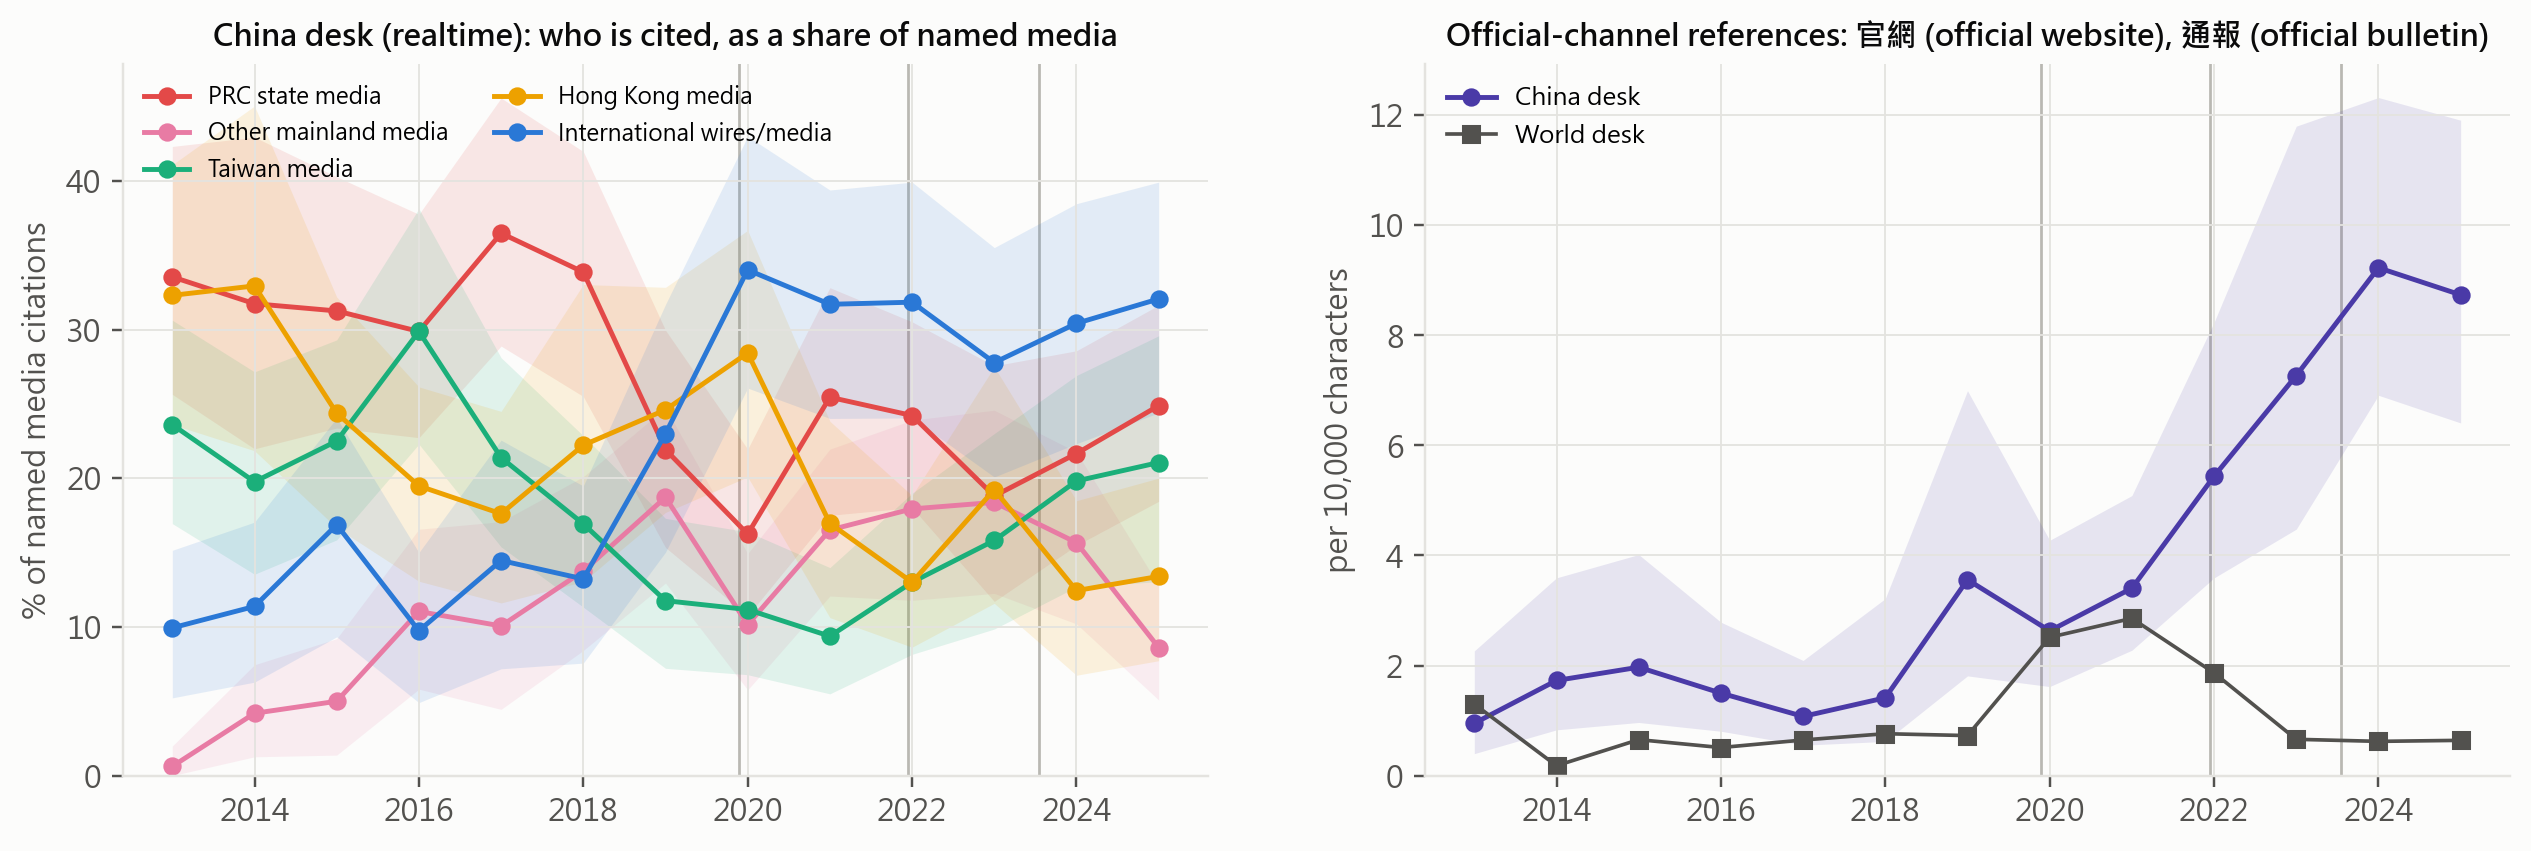
\includegraphics[width=\textwidth]{fig10_sources.png}
\caption{Sources on the China desk, realtime corpus. The left panel shows each group's share of named media citations. The right panel shows references to official channels (官網 ``official website'', 通報 ``official bulletin'') per 10,000 characters on the China desk and the World desk. Bands are 95\% confidence intervals.}
\label{fig:sources}
\end{figure}

\begin{table}[tbp]
\centering
\small
\begin{tabular}{@{}lccc@{}}
\toprule
Source group & 2013--2018 & 2019--2021 & 2022--2025 \\
\midrule
Chinese state media & 33 (30--37) & 21 (16--25) & 22 (19--25) \\
International wires and media & 13 (10--17) & 30 (23--34) & 31 (28--32) \\
Hong Kong media & 25 (18--33) & 23 (17--28) & 15 (12--19) \\
Taiwanese media & 22 (17--30) & 11 (9--12) & 17 (13--21) \\
Other mainland media & 7 (1--14) & 15 (10--19) & 15 (9--18) \\
\bottomrule
\end{tabular}
\caption{Average share (\%) of named media citations on the China desk, realtime corpus, with the range of yearly values in parentheses.}
\label{tab:shares}
\end{table}

These patterns do not fit the idea of a paper that copies Chinese state media. If anything, the China desk cites state media less and international wires more than it did ten years ago. What changed is that more of its reporting is based on what Chinese institutions announce directly. That is closer to the \textit{Washington Post}'s actual concern, which was about whose account of events the paper relays, than any measure of tone. There are other explanations, though. Chinese government bodies have moved more of their announcements to official websites and social media accounts, foreign journalists' access to China shrank sharply after 2020, and two independent Hong Kong outlets, \textit{Apple Daily} and \textit{Stand News}, closed in 2021. The robustness checks rule out the pandemic as the main driver, but I cannot separate the remaining explanations with the data in this study.

\section{Summary of findings}

\begin{table}[tbp]
\centering
\small
\begin{tabular}{@{}p{0.2\textwidth}p{0.36\textwidth}p{0.36\textwidth}@{}}
\toprule
Question & Hypothesis & Finding \\
\midrule
Q1 Divergence & China desk moves away from the World desk after Dec 2021 & Not supported. AUC rise not significant after correction; on the pre-2021 axis, both desks moved together and their distance did not change. \\
Q2 Convergence & China desk moves toward the Singapore desk after Dec 2021 & Not at the restructuring. Gradual partial convergence in style beginning about 2019--2020; no break. \\
Q3 Stance & China desk hedges less and uses more obligation words, increasingly after Dec 2021 & Hedges less (by a fifth to a third even within topic), but for twenty years; fewer obligation words, not more; no change at Dec 2021. Weak evidence of more boosters. \\
Sources (exploratory) & -- & Official bulletins and websites roughly tripled relative to the World desk after Dec 2021, robust to COVID; state-media share fell. \\
\bottomrule
\end{tabular}
\caption{Answers to the research questions.}
\label{tab:summary}
\end{table}

None of the three hypotheses about how the China desk writes is supported as a change at the restructuring (Table~\ref{tab:summary}). Two long-run features of the desk are real: it hedges less than the World desk, and its style has slowly become less distinctive. The only change that looks like a break is in sourcing.

\section{Limitations}

\begin{itemize}
\item \textbf{The archive:} The Wayback Machine holds what its crawlers saved. The paywall leaves me with only the leads of most desk articles from 2016 to 2023. Leads are short (about 60 words), so estimates from them are noisy, especially for rare categories such as boosters.
\item \textbf{Genre:} Realtime news and desk articles differ in length and purpose. I report them separately and never compare their levels.
\item \textbf{The control desk:} The World desk has its own news shocks, such as the wars in Ukraine and Gaza. The year-level tests, the fixed-axis test and the extra comparison desks reduce this problem but do not remove it, and one result (realtime obligation) depends on which desk is the control.
\item \textbf{Few years after the break:} Only four years follow December 2021, so year-level tests have little power, and a trend that starts a year or two early cannot be told apart from a break.
\item \textbf{Ambiguous words:} 應該 (``should'' or ``probably'') and 可以 (``may'' or ``can'') each have two meanings, and word segmentation is never perfect. The per-word results let readers judge each word on its own.
\item \textbf{Topics:} The topic model assigns each article one topic, which is a coarse summary, and the share of the hedging gap it explains depends on the number of topics (a fifth to a half). That a substantial gap remains in every version is the robust part of the result.
\item \textbf{Counting sources:} Counting outlet names misses unnamed sources and can include mentions that are not citations. 通報 can also be a verb meaning ``to notify''. A hand-coded sample would be needed to measure how precise the source counts are.
\item \textbf{Causation:} None of these designs identifies a cause. The restructuring, the pandemic and changes in Chinese and Hong Kong media all happened within the same few years.
\end{itemize}

\section{Conclusion}

The computational evidence does not support the idea that Zaobao's China desk changed its tone after the 2021 restructuring or the 2023 \textit{Washington Post} report. The desk's lower hedging is a feature of the last twenty years, not of the last four, and it persists when articles on the same topic are compared. The desk is no more prescriptive than the World desk, and its style has drifted slowly toward the rest of the paper since about 2019 rather than turning toward the Singapore desk at a particular moment.

What did change is where the China desk gets its information. After 2021, it relied much more on official bulletins and official websites, even as its use of Chinese state media declined, and this change outlasted the pandemic. The question of whether Zaobao ``echoes Beijing'' may therefore have less to do with how the paper writes than with whose announcements it reports. Testing that properly would need a hypothesis stated before looking at the data, a hand-coded sample of sources, and a comparison with other Chinese-language outlets in the region, such as Hong Kong's \textit{Ming Pao} or Malaysia's \textit{Sin Chew Daily}. That comparison would separate Zaobao's own choices from changes in what Chinese authorities publish and what foreign reporters can access.

\begin{thebibliography}{99}
\small
\sloppy
\bibitem{sph100} SPH Media. (2024, January 22). \textit{100 years later: What's new with Lianhe Zaobao?} \url{https://www.sph.com.sg/trade-highlights/features/100-years-later-whats-new-with-lianhe-zaobao}
\bibitem{sphhistory} SPH Media. (2024, July 31). \textit{Our history.} \url{https://www.sph.com.sg/our-history}
\bibitem{zaobao} 聯合早報. (n.d.). \textit{首頁 | 聯合早報} [Homepage | Lianhe Zaobao]. \url{https://www.zaobao.com.sg}
\bibitem{thinkchina} ThinkChina. (n.d.). \textit{About ThinkChina.} \url{https://www.thinkchina.sg/about-us}
\bibitem{ho2022} Ho, G. (2022, February 17). SPH to restructure media business into not-for-profit entity to support quality journalism. \textit{The Straits Times.} \url{https://www.straitstimes.com/singapore/sph-to-restructure-media-business-into-not-for-profit-entity}
\bibitem{gan2021} Gan, N., \& Xiong, Y. (2021, November 3). Chinese tennis star accuses former top government leader of sexual assault. \textit{CNN.} \url{https://www.cnn.com/2021/11/03/china/china-metoo-peng-shuai-zhang-gaoli-intl-hnk/index.html}
\bibitem{gu2021} Gu, G. (2021, December 20). Zaobao exclusive video interview: Peng Shuai says she made no claims of sexual assault. \textit{ThinkChina.} \url{https://www.thinkchina.sg/society/zaobao-exclusive-video-interview-peng-shuai-says-she-made-no-claims-sexual-assault}
\bibitem{mahtani2023} Mahtani, S., \& Chandradas, A. (2023, July). Singapore's Chinese-language newspaper increasingly echoes China's message. \textit{The Washington Post.} \url{https://www.washingtonpost.com/world/interactive/2023/singapore-china-news-influence-lianhe-zaobao/}
\bibitem{lui2023} Lui, T. Y. (2023, August 5). \textit{Letter to the editor, The Washington Post.} Ministry of Foreign Affairs Singapore. \url{https://www.mfa.gov.sg/Overseas-Mission/Washington/Mission-Updates/2023/08/Letter-to-the-Editor---Washington-Post}
\bibitem{palmer} Palmer, F. R. (2001). \textit{Mood and modality} (2nd ed.). Cambridge University Press.
\bibitem{hyland} Hyland, K. (1998). \textit{Hedging in scientific research articles.} John Benjamins.
\bibitem{jieba} Sun, J. (2012). \textit{jieba: Chinese text segmentation} [Computer software]. \url{https://github.com/fxsjy/jieba}
\bibitem{wooldridge} Wooldridge, J. M. (1999). Distribution-free estimation of some nonlinear panel data models. \textit{Journal of Econometrics, 90}(1), 77--97.
\bibitem{santos} Santos Silva, J. M. C., \& Tenreyro, S. (2006). The log of gravity. \textit{The Review of Economics and Statistics, 88}(4), 641--658.
\bibitem{nmf} Lee, D. D., \& Seung, H. S. (1999). Learning the parts of objects by non-negative matrix factorization. \textit{Nature, 401}(6755), 788--791.
\bibitem{cameron} Cameron, A. C., \& Miller, D. L. (2015). A practitioner's guide to cluster-robust inference. \textit{Journal of Human Resources, 50}(2), 317--372.
\bibitem{monroe} Monroe, B. L., Colaresi, M. P., \& Quinn, K. M. (2008). Fightin' words: Lexical feature selection and evaluation for identifying the content of political conflict. \textit{Political Analysis, 16}(4), 372--403.
\bibitem{bh} Benjamini, Y., \& Hochberg, Y. (1995). Controlling the false discovery rate: A practical and powerful approach to multiple testing. \textit{Journal of the Royal Statistical Society: Series B, 57}(1), 289--300.
\bibitem{massey} Massey, B. L., \& Chang, L. A. (2002). Locating Asian values in Asian journalism: A content analysis of web newspapers. \textit{Journal of Communication, 52}(4), 987--1003.
\bibitem{hanitzsch} Hanitzsch, T., Hanusch, F., Ramaprasad, J., \& de Beer, A. S. (Eds.). (2019). \textit{Worlds of journalism: Journalistic cultures around the globe.} Columbia University Press.
\bibitem{wong} Wong, K. (2004). Asian-based development journalism and political elections: Press coverage of the 1999 general elections in Malaysia. \textit{Gazette, 66}(1), 25--40.
\end{thebibliography}

\end{document}
